\documentclass[10pt,twocolumn,letterpaper]{article}

\usepackage{iccv}
\usepackage{times}
\usepackage{epsfig}
\usepackage{graphicx}
\usepackage{color}
\usepackage{caption}
\usepackage{amsmath}
\usepackage{amssymb}
\usepackage{bm}
\usepackage{booktabs}
\usepackage{lib}
\usepackage{algorithm}
\usepackage{algpseudocode}
 
\algnewcommand{\Initialize}[1]{%
  \State \textbf{Initialize:}
  \Statex \parbox[t]{\linewidth}{\raggedright #1}
}

\usepackage[pagebackref=true,breaklinks=true,letterpaper=true,colorlinks,bookmarks=false]{hyperref}

\iccvfinalcopy % *** Uncomment this line for the final submission

\def\iccvPaperID{1772} % *** Enter the ICCV Paper ID here
\def\httilde{\mbox{\tt\raisebox{-.5ex}{\symbol{126}}}}

% Pages are numbered in submission mode, and unnumbered in camera-ready
\ificcvfinal\pagestyle{empty}\fi
\begin{document}

%%%%%%%%% TITLE
\title{Amodal Completion and Size Constancy in Natural Scenes}
%\title{Object Size from a Single Image}

\author{Abhishek Kar, Shubham Tulsiani, Jo\~{a}o Carreira and Jitendra Malik\\
University of California, Berkeley - Berkeley, CA 94720\\
{\tt\small \{akar,shubhtuls,carreira,malik\}@eecs.berkeley.edu}}

\maketitle
%\thispagestyle{empty}

\begin{abstract}

% work in progress
We address the problem of fully automatic object localization and reconstruction from a single image. This is both a very challenging and very important problem which has, until recently, received limited attention due to difficulties in segmenting objects and predicting their poses. Here we leverage recent advances in learning convolutional networks for object detection and segmentation and introduce a complementary network for the task of camera viewpoint prediction. These predictors are very powerful, but still not perfect given the stringent requirements of shape reconstruction. Our main contribution is a new class of deformable 3D models that can be robustly fitted to images based on noisy pose and silhouette estimates computed upstream and that can be learned directly from 2D annotations available in object detection datasets. Our models capture top-down information about the main global modes of shape variation within a class providing a ``low-frequency'' shape. In order to capture fine instance-specific shape details, we fuse it with a high-frequency component recovered from shading cues. A comprehensive quantitative analysis and ablation study on  the PASCAL 3D+ dataset validates the approach as we show fully automatic reconstructions on PASCAL VOC as well as large improvements on the task of viewpoint prediction.


\end{abstract}

\vspace{-0.2cm}
\section{Introduction}
\vspace{-0.2cm}

Despite being massively over-parameterized, deep neural networks with billions of parameters still learn representations that generalize well when trained with supervised and unsupervised learning approaches. This is despite the classical notions of overfitting when provided with many parameters. A widely held consensus is that deep networks find simple solutions that generalize due to various \emph{implicit} regularization effects~\citep{blanc2020implicit,woodworth2020kernel,arora2018optimization,gunasekar2017implicit,wei2019regularization,li2019towards}. Does this mean that large, over-parameterized networks will also be simpliarly performant for offline RL, scaling and generalizing well as the number of parameters is increased?

In the first part of this chapter, we show that, implicit regularization may lead to poor learned representations when training overparameterized deep network value functions via offline RL. This often manifests as the inability to improve performance with larger deep network models, and in particular, unreliable optimization behavior over the course of offline RL training. While there is already some empirical studies showing that value function training via offline temporal-difference (TD) learning leads to emergence of poor representations~\citep{kumar2021implicit}, our goal in this chapter is to understand the cause in a simpler theoretical model and develop a potential solution. Building on the theoretical framework developed by \citet{blanc2020implicit,damian2021label}, we characterize the implicit regularizer that arises when training deep value functions with offline TD learning. The form of this implicit regularizer implies that offline TD-learning would ``co-adapt'' the learned feature representations at state-action tuples that appear on either side of a Bellman backup.

Practically, we illustrate that this theoretically-predicted co-adaptation phenomenon results in a higher dot product of the features of consecutive state-action tuples learned by the Q-value network~(\Secref{sec:problem}). Training runs that exhibit feature co-adaptation typically converge to poorly performing solutions. Even when Q-values are not overestimated, prolonged training in offline RL can result in performance degradation as feature co-adaptation increases. To mitigate this co-adaptation issue, which arises as a result of implicit regularization, we propose an \emph{explicit regularizer} that we call \drmethodname~(\Secref{sec:method}). While exactly estimating the effects of the theoretically derived implicit regularizer is computationally difficult, \drmethodname\ provides a simple and tractable approximation that mitigates the issues discussed above. In practice, \drmethodname\ amounts to regularizing the features at consecutive state-action pairs to be dissimilar in terms of their dot-product similarity. Empirically, we find that \drmethodname\ prevents previously noted pathologies such as feature rank collapse~\citep{kumar2021implicit}, gives methods that train for longer and improves performance relative to the base offline RL method on benchmark problems.

Building on this approach, in the second part of this chapter, we perform a large-scale empirical study that aims to train a large model via offline conservative Q-learning. Specifically, we train a single policy to play 40 Atari games~\citep{bellemare2013arcade}, similarly to \citet{lee2022multi}, and evaluate performance when the training dataset contains expert trajectories \emph{and} when the data is sub-optimal. This problem is especially challenging because of the diversity of games with their own unique dynamics, reward, visuals, and agent embodiments. Furthermore, the sub-optimal data setting requires the learning algorithm to ``stitch together'' useful segments of sub-optimal trajectories to perform well. Our approach, \textbf{scaled Q-learning}, incorporates a variant of the \drmethodname\ technique which normalizes features instead of regularization to attain the same benefit without needing a hyperparameter, in conjunction with careful neural network architectural design decisions. Scaled Q-learning is able to train upto 80 million parameter ResNet~\citep{he2016resnet} models entirely via offline RL and the performance of our approach follows a power-law relationship between model capacity and performance, similar to various scaling studies in supervised and unsupervised learning. In terms of absolute performance, scaled Q-learning learns policies that attain more than 100\% human-level performance on most of the 40 games, about \textbf{2x} better than prior supervised learning~(SL) approaches for learning from sub-optimal offline data (51\% human-level performance).    

% Our first contribution is the derivation of the implicit regularizer that arises when training deep net value functions via TD learning, and an empirical demonstration that it manifests as \emph{feature co-adaptation} in the offline deep RL setting.
% %, which results in highly similar feature representations for state-action tuples at consecutive time steps. 
% Feature co-adaptation accounts at least in part for some of the challenges of offline deep RL, including degradation of performance with prolonged training. Second, we propose a simple and effective \emph{explicit} regularizer for offline value-based RL, \drmethodname, which minimizes the feature similarity between state-action pairs appearing in a bootstrapping update. \drmethodname\ is inspired by the theoretical derivation of the implicit regularizer, it alleviates co-adaptation and can be easily combined with modern offline RL methods, such as REM~\citep{agarwal2019optimistic}, CQL~\citep{kumar2020conservative}, and BRAC~\citep{wu2019behavior}. Empirically, using \drmethodname\ in conjunction with existing offline RL methods provides about \textbf{60\%} performance improvement on the harder D4RL~\citep{fu2020d4rl} tasks, and \textbf{160\%} and \textbf{25\%} stability gains for REM and CQL, respectively, on offline RL tasks in 17 Atari 2600 games. Additionally, we observe large improvements on image-based robotic manipulation tasks~\citep{singh2020cog}.

%\vspace{-0.2cm}
\section{Related Work}
\label{sec:related}
\vspace{-0.2cm}

Errors arising from inadequate sampling, distributional shift, and function approximation have been rigorously studied as ``error propagation'' in approximate dynamic programming (ADP)~\citep{bertsekas1996ndp,munos2003errorapi,farahmand2010error,bruno2015approximate}. These works often study how Bellman errors accumulate and propagate to nearby states via bootstrapping. In this chapter, we build upon tools from this analysis to show that performing Bellman backups on static datasets leads to error accumulation due to out-of-distribution values. Our approach is motivated as reducing the rate of propagation of error propagation between states.

BEAR constrains actor updates so that the actions remain in the support of the training dataset. Several works have explored similar ideas in the context of off-policy learning learning in online settings. \citet{kakade2002cpi} shows that large policy updates can be destructive, and propose a conservative policy iteration scheme which constrains actor updates to be small for provably convergent learning. \citet{grau-moya2018soft} use a learned prior over actions in the maximum entropy RL framework~\citep{levine2018rlasinference} and justify it as a regularizer based on mutual information. However, none of these methods use static datasets. Importance Sampling based distribution re-weighting~\cite{munos2016safe,gelada2019off,precup2001offpol,mahmood2015emphatic} has also been explored primarily in the context of off-policy policy evaluation.

Most closely related to our approach is batch-constrained Q-learning (BCQ)~\citep{fujimoto2018off} and SPIBB~\citep{laroche2019spibb}, which also discuss instability arising from previously unseen actions. \citet{fujimoto2018off} show convergence properties of an action-constrained Bellman backup operator in tabular, error-free settings. We prove stronger results under approximation errors and provide a bound on the \emph{suboptimality} of the solution. This is crucial as it drives the design choices for a practical algorithm. As a consequence, although we experimentally find that \citep{fujimoto2018off} outperforms standard Q-learning methods when the off-policy data is collected by an expert, BEAR outperforms \cite{fujimoto2018off} when the off-policy data is collected by a suboptimal policy, as is common in real-life applications. SPIBB~\citep{laroche2019spibb}, like BEAR, is an algorithm based on constraining the learned policy to the support of a behavior policy. However, the authors of SPIBB do not extend safe performance guarantees from the batch-constrained case to the relaxed support-constrained case, and do not study high-dimensional control tasks. 
% REM~\citep{agarwal19striving} is a concurrent work that uses a random convex combination of an ensemble of Q-networks to perform offline reinforcement learning from a static dataset consisting of interaction data generated while training a DQN agent.

\documentclass[../thesis.tex]{subfiles}

\begin{document}

%%%%%%%%% TITLE
% \title{Amodal Completion and Size Constancy in Natural Scenes}
\blfootnote{This chapter is based on joint work with Shubham Tulsiani, Jo{\~{a}}o Carreira and Jitendra Malik \cite{amodalKarTCM15}, presented primarily as it appears in the ICCV 2015 proceedings. Statements throughout the chapter (such as references to ``prior work'') should be read with this context in mind.}
% \begin{abstract}
%Towards the goal of enabling vision systems to reason with models of scenes inferred from a single image,  we study the task of enriching recognition system descriptions  with veridical sizes and relative depths of all the objects. 

We consider the problem of enriching current object detection systems with veridical object sizes and relative depth estimates from a single image. There are several technical challenges to this, such as occlusions, lack of calibration data and the scale ambiguity between object size and distance. These have not been addressed in full generality in previous work. Here we propose to tackle these issues by building upon advances in object recognition and using recently created large-scale datasets. We first introduce the task of amodal bounding box completion, which aims to infer the the full extent of the object instances in the image. We then propose a probabilistic framework for learning category-specific object size distributions from available annotations and leverage these in conjunction with amodal completions to infer veridical sizes of objects in novel images. Finally, we introduce a focal length prediction approach that exploits scene recognition to overcome inherent scale ambiguities and demonstrate qualitative results on challenging real-world scenes.
\end{abstract}
In Chapter \ref{chapter:CategoryShapes}, we tackled the problem of learning object shape distributions and automatically localizing and  reconstructing them in scenes. However, these object reconstructions are independent of each other, i.e. the relative sizes and depths of the objects are not taken into acount at all. In this chapter, we present ideas which allow us to take our object reconstructions from the previous chapter and assemble a coherent scene with them.

Consider \figref{fig1}. Humans can effortlessly perceive two chairs of roughly the same height and tell that one is much closer than the other, though still further away than the person, who is taller than the chairs. Compare this to what a state-of-the-art object detector tells us about the image: that there are two chairs, 120 and 40 pixels tall, and one person with 200 pixels from top to bottom. How can we enable computer vision systems to move beyond this crude 2D representation and allow them to capture richer models of their environments, such as those that humans take for granted?

The 3D world is a lot more structured than it looks like from the retina (or from a camera sensor), where objects jump around with each saccade and grow and shrink as we move closer or farther from them. We do not perceive any of this because our brains have learned priors about how visual inputs correlate with the underlying environment, and this allows us to directly access realistic and rich models of scenes. The priors we use can be categorized as being related to either \textit{geometry} or \textit{familiarity}.

\begin{figure}[t!]
  \centering
  \includegraphics[width=.9\textwidth]{figures/amodal/Fig_1.png} % COCO_train2014_000000352357.jpg
  \caption{\figlabel{fig1} Perceiving the veridical size of objects in realistic scenes, from a single image, requires disentangling size and depth, being able to compensate for occlusions and to determine intrinsic camera parameters. We tackle all three of these problems, leveraging recent developments in object recognition and large annotated object and scene datasets.}
\end{figure}

Image projection properties, such as the fact that the distance of an object from the camera dictates apparent size and that parallel lines in the scene vanish in the image, provide useful signal for perceiving structure. Familiarity cues are complementary and impose expectations on individual objects and configurations -- we expect most objects to be supported by another surface and we have the notion of \textit{familiar size} -- similar objects are of similar sizes. In this chapter, we exploit geometry and familiarity cues and develop a framework to build richer models of the visual input than those given by current computer vision systems, which are still largely confined to the 2D image plane.

The notion that certain geometrical cues can aid perception has been known since the time of Euclid - the points in the image where objects touch the ground together with their perceived heights allows inference of real world object size ratios \cite{burton45}. Familiarity cues, on the other hand must be learned, which can be done using available annotations and building upon rapid recent progress in object recognition, more robustly harnessed to explain novel images. Similar ideas have been proposed by Hoiem \etal~\cite{hoiem2008putting,Hoiem:book} and Gupta \etal ~\cite{gupta2010blocks} who studied the interaction between object detection and scene layout estimation and showed that, by reasoning over object sizes within their 3D environment, as opposed to within the image, one could perform better object detection. Lalonde \etal~\cite{lalonde2007photo} and Russell \etal~\cite{russell2009building} also tackled a problem similar to operationalizing size constancy and inferred object sizes of annotated objects. These works, while sharing similar goals to ours, were limited in their scope as they assumed fully visible instances - object recognition technology at the time being a limiting factor. In this chapter, we aim for veridical size estimation in more realistic settings -- where occlusions are the rule rather than the exception. Occlusions present a significant technical challenge as they break down a number of assumptions(\eg in 
\figref{fig1} not modeling occlusions would yield an incorrect estimate of the relative depths of the two chairs shown).

To overcome these challenges, we first introduce amodal completion. This is a very well studied ability of human perception, primarily in the context of amodal edge perception \cite{kanizsa1979organization}, building on theories of \textit{good continuation} \cite{shipley2001fragments}. In the context of objects, amodal completion manifests itself as inference of the complete shape of the object despite visual evidence for only parts of it \cite{breckon2005amodal}.
%Psychology: Do Artists See Their Retinas? Cavanagh
%Amodal completion: Amodal volume completion: 3D visual completion. Fisher
%Organization in vision: Essays on Gestalt perception. Kanizsa 1979
In \secref{amodalCompletion}, we tackle the amodal completion task and frame it as a recognition problem, formalized as  predicting the full extent of object bounding boxes in an image, as opposed to only the visible extent. We build amodal extent predictors based on convolutional neural networks which we train on the challenging PASCAL VOC dataset. In \secref{sizeconstancy}, we propose a formulation that, leveraging amodally completed objects, can disentangle relative object sizes and object distances to the camera. This geometric reasoning allows us only to infer distances for objects up to a scaling ambiguity in each image. To overcome this ambiguity, we show in \secref{sceneFocal} that it is possible to leverage statistical dependencies between scenes and intrinsic camera parameters, and learn to predict focal lengths of scenes from large scale scene datasets. Finally, we present qualitative  results exhibiting veridical size estimation in complex scenes.

%The 3D world is a lot less wild than it looks like from the retina or from a camera sensor. In the retina, due to saccades, objects jump around several times per second. They also grow as we get closer, and get smaller as we move away. The ability to factor out such artifacts of seeing from the true nature of the scenes being seen is called \textit{visual constancy} and makes possible a more seamless interaction of an agent with its environment.


%Computer vision systems are still largely confined to the image plane. For example, in fig. \ref{fig1}, a state-of-the-art object detector localizes three people having heights of 100, 70 and 140 pixels, instead of three people of approximately the same height. Support relationships provide important cues for size constancy by leveraging time-proven Euclidean geometry: the points in the image where objects touch the ground together with their perceived heights allows inference of real world object size ratios \cite{}. Another important cue is familiarity (recognition). As an example, face sizes vary within a narrow range, so their dimensions in the image are informative of nearness to the camera.

%[Say something about size from familiarity (recognition)]

%Both types of cues are affected by occlusions, which translate into depth distortions, but have not yet been considered in prior art \cite{}. In this paper we tackle the size constancy problem in more generality, in realistic settings -- where occlusions are the rule rather than the exception -- by introducing amodal completion. We introduce amodal completion predictors based on convolutional networks which we train on especially engineered datasets having both natural and synthetic occlusion patterns. Additionally, we propose a formulation that, leveraging amodal completion, can disentangle relative class sizes and object distances to the camera from  training data having just ground truth bounding boxes and class labels. Finally, we present qualitative detection results exhibiting size constancy in complex Microsoft COCO scenes. 



%\section{Related Work}


Hoiem et al \cite{hoiem2008putting} studied the interaction between object detection and scene layout estimation and showed that reasoning over object sizes within their 3D environment, as opposed to within the image, had a positive impact on detection performance. 

The work Lalonde et al \cite{lalonde2007photo} is close to ours. It estimates average real world sizes of many object categories in the 3D world, from annotated LabelMe data.

This was still in the HOG age  \cite{dalal2005histograms} -- here we leverage the more powerful feature extraction technology we have now to be able to widthstand occlusions and recover metric information.

Building a database of 3d scenes from user annotations \cite{russell2009building}. This is a heavy duty system with quite a broad model, that classifies pairwise relationships into support, attachment, occlusion, etc. On the bright side it assumes every pixel is annotated as belonging in a region. It also does not perform completion and it's not clear  exactly how they recover depth of occluded objects, probably using familiarity, etc.. ?
 
 Other references:
-  Are Cars Just 3D Boxes? – Jointly Estimating the 3D Shape of Multiple Objects. Schindler
-  Towards Scene Understanding with Detailed 3D Object Representations. Schindler
------------------------------------------------------

Psychology:
Do Artists See Their Retinas? Cavanagh

Amodal completion:
Amodal volume completion: 3D visual completion. Fisher


Organization in vision: Essays on Gestalt perception. Kanizsa 1979

%
\section{Amodal Completion}
\seclabel{amodalCompletion}
\setlength{\epigraphwidth}{.9\textwidth}
\epigraph{``Almost \textit{nothing} is visible in its entirety, yet almost \textit{everything} is perceived as a whole and complete"}{\textit{Stephen Palmer}}

Classic computer vision approaches have traditionally been impoverished by trying to explain just what we see in an image. For years, standard benchmarks have focused on explaining the visible evidence in the image - not the world behind it. For example, the well-studied task of predicting the bounding box around the visible pixels of an object has been the goal of current object detection systems. As humans, not only can we perceive the visible parts of the chair depicted in \figref{fig1}, we can confidently infer the full extent of the actual chair.

This representation of objects, that humans can effortlessly perceive, is significantly richer than what current systems are capable of inferring. We take a step forward towards achieving similar levels of understanding by attacking the task of perceiving the actual extent of the object, which we denote as \textit{amodal completion}. The amodal representation of objects enables us to leverage additional scene information such as support relationships, occlusion orderings \etc For example, given the amodal and visible extents of two neighboring objects in the image, one can figure out if one is occluded by the other. Explicitly modeling amodal representations also allow us to implicitly model occlusions patterns rather than trying to ``explain them away" while detecting objects. As described in \secref{sizeconstancy}, we can use these representations to infer real world object sizes and their relative depths just from images.

The primary focus of object recognition systems \cite{girshick2013rich,felzens_latent_pami10} has been to localize and identify objects, despite occlusions, which are usually handled as noise. Several recently proposed recognition systems do explicitly model occlusion patterns along with detections and provide a mechanism for obtaining amodal extent of the object \cite{ghiasi2014parsing, xiang_cvpr15, zia2014towards}. However, these approaches have been shown to work only on specific categories and rely on available shape models or depth inputs, for learning to reason over occlusions. In contrast, we aim to provide a generic framework that is not limited by these restrictions. Our proposed framework is described below.

\subsection{Learning to Predict Amodal Boxes}
Given a candidate visible bounding box, we tackle the task of amodal completion -- the input to our system is some modal bounding box (\eg obtained via a detection system) and we aim to predict the amodal extent for the object. We frame this task as predicting the amodal bounding box, which is defined as  the bounding box of an object in the image plane if the object were completely visible, \ie if inter-object occlusions and truncations were absent. The problem of amodal box prediction can naturally be formulated as a regression task - given a noisy modal bounding box of an object we regress to its amodal bounding box coordinates. The amodal prediction system is implicitly tasked with learning common occlusion/truncation patterns and their effects on visible object size. It can subsequently infer the correct amodal coordinates using the previously learned underlying visual structure corresponding to occlusion patterns. For example, the learner can figure out that chairs are normally vertically occluded by tables and that it should extend the bounding box vertically to predict the full extent of the chair.

Let $b = (x,y,w,h)$ be a candidate visible (or modal) bounding box our amodal prediction system receives ($(x,y)$ are the co-ordinates of the top-left corner and $(w,h)$ are the width and height of the box respectively) and $b^* = (x^*,y^*,w^*,h^*)$ be the amodal bounding box of the corresponding object, our regression targets are $(\frac{x-x^*}{w},\frac{y-y^*}{h},\frac{(x+w)-(x^*+w^*)}{w},\frac{h-h^*}{h})$. Our choice of targets is inspired by the fact that for the $y$ dimension, the height and bottom of the box are the parameters we actually care about (see \secref{sizeconstancy}) whereas along the $x$ dimension the left co-ordinate is not necessarily more important than the right.

\paragraph{Learning:} We use a Convolutional Neural Network (CNN) \cite{neocognitron,Lecun89} based framework to predict the co-ordinates of the amodal bounding box. The hypothesis is that the amodal prediction task can be reliably addressed given just the image corresponding to the visible object region -- seeing the left of a car is sufficient to unambiguously infer the full extent without significantly leveraging context. Based on this observation, we extract from input image $I$, the region corresponding to the detection box $b$ and train the CNN using targets derived as above from the amodal box $b^*$. We impose an $L_2$ penalty on the targets and regress from the extracted CNN image features to the targets. We initialize our model using the AlexNet \cite{krizhevsky2012imagenet} CNN pretrained for Imagenet \cite{imagenet_cvpr09} classification and then finetune the model specific to our task using backpropagation. Training is carried out with jittered instances of the ground truth bounding box to enable generalization from noisy settings such as detection boxes and also serve as data augmentation.

We train two variants of the above network - class-specific and class agnostic. Both these systems comprise of 5 convolutional layers followed by 3 fully-connected layers. The class-specific network has separate outputs in the last layers for different classes and is trained with positive examples from a specific class whereas the class agnostic network has a single set of outputs across all classes. Intuitively, the class-specific network learns to leverage occlusion patterns specific to a particular class (\eg chair occluded by a table) whereas the class agnostic network tries to learn occlusion patterns common across classes. Another argument for a class agnostic approach is that it is unreasonable to expect annotated amodal bounding box data for a large number of categories. A two-stage system, where we first predict the visible bounding box candidates and then regress from them to amodal boxes, enables leveraging these class agnostic systems to generalize to more categories. As we demonstrate in \secref{sizeconstancy}, this class agnostic network can be applied to novel object categories to learn object sizes.

\begin{figure}
  \centering
  \includegraphics[width=.9\linewidth]{figures/amodal/Amodal.png}
  \caption{\figlabel{amodal} Generating amodal bounding boxes for instances in PASCAL VOC. We use the 3D models aligned to images from the PASCAL 3D+ \cite{pascal3d} and render them with their annotated 3D pose to obtain binary masks. We then use the tightest fitting bounding box around the mask as our ground truth amodal bounding box.}
\end{figure}


%\section{Experiments}
%\seclabel{experiments}
%\subsection{Amodal completion}
\subsection{Quantitative Evaluation}
\paragraph{Dataset:} For the purpose of amodal bounding box prediction, we need annotations for amodal bounding boxes (unlike visible bounding box annotations present in all standard detection datasets). We use the PASCAL 3D+~\cite{pascal3d} dataset which has approximate 3D models aligned to 12 rigid categories on PASCAL VOC~\cite{pascal-voc-2012} to generate these amodal bounding box annotations. It also contains additional annotations for images from ImageNet \cite{imagenet_cvpr09} for each of these categories (22k instances in total from ImageNet). For example, it has between 4 different models aligned to ``chair'' and 10 aligned to ``cars''. The different models primarily distinguish between subcategories (but might also be redundant). The 3D models in the dataset are first aligned coarsely to the object instances and then further refined using keypoint annotations. As a consequence, they correctly capture the amodal extent of the object and allow us to obtain amodal ground-truth.  We project the 3D model fitted per instance into the image, extract the binary mask of the projection and fit a tight bounding box around it which we treat as our amodal box (\figref{amodal}). We train our amodal box regressors on the detection training set of PASCAL VOC 2012 (\textit{det-train}) and the additional images from ImageNet for these 12 categories which have 3D models aligned in PASCAL 3D+ and test on the detection validation set (\textit{det-val}) from the PASCAL VOC 2012 dataset.

\paragraph{Experiments:} We benchmark our amodal bounding box predictor under two settings - going from ground truth visible bounding boxes to amodal boxes and in a detection setting where we predict amodal bounding boxes from noisy detection boxes. We compare against the baseline of using the modal bounding box itself as the amodal bounding box (\textit{modal bbox}) which is in fact the correct prediction for all untruncated instances. \tableref{gtBboxTable} summarizes our experiments in the former setting where we predict amodal boxes from visible ground truth boxes on various subsets of the dataset and report the mean IoU of our predicted amodal boxes with the ground truth amodal boxes generated from PASCAL 3D+. As expected, we obtain the greatest boost over the baseline for truncated instances. Interestingly, the class agnostic network performs as well the class specific one signaling that occlusion patterns span across classes and one can leverage these similarities to train a generic amodal box regressor. 

To test our amodal box predictor in a noisy setting, we apply it on bounding boxes predicted by the RCNN\cite{girshick2013rich} system from Girshick \etal. We assume a detection be correct if the RCNN bounding box has an IoU $> 0.5$ with the ground truth visible box \textit{and} the predicted amodal bounding box also has an IoU $> 0.5$ with the ground truth amodal box. We calculate the average precision for each class under the above definition of a ``correct'' detection and call it the Amodal $AP$ (or $AP^{am}$). \tableref{detectionTable} presents our $AP^{am}$ results on VOC2012 \textit{det-val}. As we can see again, the class agnostic and class specific systems perform very similarly. The notable improvement is only in a few classes (\eg diningtable and boat) where truncated/occluded instances dominate. Note that we do not rescore the RCNN detections using our amodal predictor and thus our performance is bounded by the detector performance. Moreover, the instances detected correctly by the detector tend to be cleaner ones and thus the baseline (\textit{modal bbox}) of using the detector box output as the amodal box also does reasonably well. Our RCNN detector is based on the VGG16 \cite{simonyan2014very} architecture and has a mean $AP$ of $57.0$ on the 12 rigid categories we consider.

% Latent positives table
\renewcommand{\arraystretch}{1.4}
\setlength{\tabcolsep}{6pt}
\begin{table}[htb!]
\centering
\resizebox{.5\linewidth}{!}{
\begin{tabular}{ccccc}
\toprule
& \textbf{all} & \textbf{trunc/occ} & \textbf{trunc} & \textbf{occ} \tabularnewline
\midrule

\textbf{modal bbox} & 0.66 & 0.59 & 0.52 & 0.64 \tabularnewline
\textbf{class specific} & 0.68 & 0.62 & 0.57 & 0.65 \tabularnewline
\textbf{class agnostic} & 0.68 & 0.62 & 0.56 & 0.65 \tabularnewline

\bottomrule
\end{tabular}}
\caption{Mean IoU of amodal boxes predicted from the visible bounding box on various subsets of the validation set in PASCAL VOC. Here \textit{occ} and \textit{trunc} refer to occluded and truncated instances respectively. The class specific and class agnostic methods refer to our variations of the training the amodal box regressors (see text for details) and modal bbox refers to the baseline of using the visible/modal bounding box itself as the predicted amodal bounding box.}
\tablelabel{gtBboxTable}
\end{table}

% Detection table
\renewcommand{\arraystretch}{1.4}
\begin{table*}[htb!]
\centering
\resizebox{\linewidth}{!}{
\begin{tabular}{ccccccccccccc|c}
\toprule
& \textbf{aero} & \textbf{bike} & \textbf{boat} & \textbf{bottle} & \textbf{bus} & \textbf{car} & \textbf{chair} & \textbf{table} & \textbf{mbike} & \textbf{sofa} & \textbf{train} & \textbf{tv} & \textbf{mean}\tabularnewline
\midrule

\textbf{modal bbox} & 70.0 & 66.2 & 23.9 & 35.1 & 76.4 & 57.7 & 28.9 & 24.2 & 68.3 & 45.8 & 58.1 & 59.6 & 51.2 \tabularnewline
\textbf{class specific} & 69.5 & 67.2 & \textbf{26.9} & 36.0 & \textbf{77.0} & \textbf{61.4} & \textbf{31.4} & 29.2 & \textbf{69.0} & \textbf{49.4} & \textbf{59.3} & 59.5 & \textbf{53.0} \tabularnewline
\textbf{class agnostic} & \textbf{70.0} & \textbf{67.5} & 26.8 & \textbf{36.3} & 76.8 & 61.3 & 31.1 & \textbf{30.9} & 68.9 & 48.4 & 58.6 & \textbf{59.6} & \textbf{53.0} \tabularnewline
%\midrule
% \textbf{RCNN} & 0.72 & 0.7 & 0.36 & 0.38 & 0.78 & 0.65 & 0.35 & 0.36 & 0.72 & 0.52 & 0.71 & %0.6 & 0.57 \tabularnewline
\bottomrule
\end{tabular}}
\caption{$AP^{am}$ for our amodal bounding box predictors on VOC 2012 \textit{det-val}. $AP^{am}$ is defined as the average precision when a detection is assumed to be correct only when both the modal and amodal bounding boxes have IoU $> 0.5$ with their corresponding ground truths.}
\tablelabel{detectionTable}
\end{table*}

Armed with amodal bounding boxes, we now show how we tackle the problem of inferring real world object sizes from images.

\section{Disentangling Size and Depth}
\seclabel{sizeconstancy}
Monocular cues for depth perception have been well-studied in psychology literature and there are two very important cues which emerge that tie object size and depth -  namely familiar size and relative size. Familiar size is governed by the fact that the visual angle subtended by an object decreases with distance from the observer and prior knowledge about the actual size of the object can be leveraged to obtain absolute depth of the object in the scene. Relative size, on the other hand, helps in explaining relative depths and sizes of objects - if we know that two objects are of similar sizes in the real world, the smaller object in the image appears farther. Another simple cue for depth perception arises due to perspective projection - an object further in the world appears higher on the image plane. Leveraging these three cues, we show that one can estimate real world object sizes from just images. In addition to object sizes, we also estimate a coarse viewpoint for each image in the form of the horizon and camera height. 

The main idea behind the algorithm is to exploit pairwise size relationships between instances of different object classes in images. As we will show below, given support points of objects on the ground and some rough estimate of object sizes, one can estimate the camera height and horizon position in the image - and as a result relative object depths. And in turn, given object heights in the image and relative depths, one can figure out the real world object scale ratios. Finally, exploiting these pairwise size evidences across images, we solve for absolute real world sizes (upto a common scale factor or the metric scale factor). Note that we use size and height interchangeably here as our notion of object size here actually refers to the object height.

\begin{figure}
  \centering
  \includegraphics[width=.9\textwidth]{figures/amodal/Perspective.png}
  \caption{\figlabel{perspective} Toy example illustrating our camera model and parameters. Please refer to the text for detailed explanations. }
\end{figure}

\subsection{Camera Model}
 We use a simplified perspective camera model similar to Hoiem \etal~\cite{hoiem2008putting}. Let $f$ be the focal length of the camera, $\theta_x$ the camera tilt angle along the x-axis, $h_c$ the height of the camera, $y_h$ be the horizon position in the image, $y_i^b$ be the ground support point for the $i^{th}$ object in the image and $d_i$ be the distance of the $i^{th}$ object from the camera along the camera axis ($z$ axis). We assume that the images have been corrected for camera roll and all pixel co-ordinates are with respect to the optical center (assumed to be center of the image). \figref{perspective} provides a toy illustration of our model and parameters.

Assuming that the world frame is centered at the camera with its $y$ axis aligned with the ground, the projection of a world point $\mathbf{X} = (X_w,Y_w,Z_w)$ in the image in homogeneous co-ordinates is given by:
\bes
\begin{bmatrix}
x \\
y \\
1
\end{bmatrix} = \frac{1}{Z_w}
\begin{bmatrix}
f & 0 & 0\\
0 & f & 0\\
0 & 0 & 1
\end{bmatrix}
\begin{bmatrix}
1 & 0 & 0 & 0 \\
0 & \cos\theta_x & \sin\theta_x & 0 \\
0 & -\sin\theta_x & \cos\theta_x & 0 \\
\end{bmatrix}
\begin{bmatrix}
X_w \\
Y_w \\
Z_w \\
1
\end{bmatrix}
\ees
For a world point corresponding to the ground contact point of object $i$, given by $(X_w,-h,d_i)$, its corresponding $y$ co-ordinate in the image $y_i^b$ is given by:
$
y_i^b = f\frac{(-h_c/d_i + \tan\theta_x)}{1+(h_c/d_i)\tan\theta_x}
$
Under the assumption of the tilt angle being small ($\tan\theta_x \approx \theta_x$) and height of the camera being not too large compared to object distance ($h\theta_x \ll d_i$), our approximation is 
\be
\eqlabel{groundEq}
y_i^b = -\frac{fh_c}{d_i} + f\theta_x
\ee
Here $f\theta_x$ corresponds to the position of the horizon ($y_h$) in the image. Repeating the above calculation for the topmost point of the object and subtracting from \eqref{groundEq}, we obtain
\be 
\eqlabel{sizeEq}
h_i = \frac{fH_i}{d_i}
\ee
where $h_i$ refers to the height of the object in the image and $H_i$ is the real world height of the object.
Our model makes some simplifying assumptions about the scene namely, objects are assumed to rest on the same horizontal surface (here, the ground) and camera tilt is assumed to be small. We observe that for the purpose of size inference, these assumptions turn out to be reasonable and allow us to estimate heights of objects fairly robustly.

% Algorithm box for size estimation
\begin{algorithm}[h]
\caption{Object Size Estimation}
\begin{algorithmic}
\Initialize{Initial size estimates $\mathbf{H}$ and cluster assignments}
\While {not converged}
\ForAll{images $k \in $ Dataset }
\State $(h_c,y_h) \gets $ SolveLeastSquares($y_b,h,\mathbf{H}$)
\ForAll{pairs $(i,j)$ of objects in $k$}
\State $\frac{H_i}{H_j} \gets \frac{h_i}{h_j}\frac{y_j^b-y_h}{y_i^b-y_h}$\Comment{$(1)$}
\EndFor
\EndFor
\State $\log \mathbf{H} \gets$ least squares with pairwise constraints ($1$)
\State GMM cluster log scales ($\log \mathbf{H}$)
\State Reassign objects to clusters
\EndWhile
\end{algorithmic}
\label{alg:sizeEstimation}
\end{algorithm}

\subsection{Inferring Object Sizes} 
The important observation here is that the sizes of objects in an object category are not completely random - they potentially follow a multimodal distribution. For example, different subcategories of boats may represent the different modes of the size distribution. Given some initial sizes and size cluster estimates, our algorithm for size estimation (Algorithm \ref{alg:sizeEstimation}) works by estimating the horizon and camera height per image (by solving a least squares problem using \eqref{groundEq} and \eqref{sizeEq} for all the objects in an image). With the horizon and height estimated per image, we obtain pairwise height ratios $\frac{H_i}{H_j} = \frac{h_i}{h_j}\frac{y_j^b-y_h}{y_i^b-y_h}$ for each pair of objects in an image. We obtain multiple such hypotheses across the dataset which we use to solve a least squares problem for $\log \mathbf{H}$ - the log height for each size cluster. Finally, we cluster the log sizes obtained in the previous step to obtain new size clusters and iterate. Note that $\mathbf{H}$ refers to the vector with heights of various classes and $H_i$ refers to the real world size of the $i^{th}$ object.

This particular model is equivalent to solving a latent variable model where the latent variables are the cluster memberships of the instances, the estimated variables are heights corresponding to the size clusters and the horizon and camera height for each image. The loss function we try to minimize is the mean squared error between the ground contact point predicted by the model and the amodal bounding box. Finally, the log of the object heights are assumed to be a Gaussian mixture. This final assumption ties in elegantly with psychophysics studies which have found that our mental representation of object size (referred to as assumed size~\cite{ittelson1951size,baird1963retinal,epstein1963influence}) is proportional to the logarithm of the real world object size~\cite{konkle2011canonical}.

Our image evidences in the above procedure include the ground support points and heights for all the objects in the image. Note that amodal bounding boxes for objects provide us exactly this information. They account for occlusions and truncations and give us an estimate of the full extent of the object in the image. The above algorithm with occluded/truncated visible bounding boxes would fail miserably and we use our amodal bounding box predictor to first ``complete'' the bounding boxes for us before using our size inference algorithm to infer object heights.

\begin{figure}[htb]
  \centering
  \includegraphics[width=.9\textwidth]{figures/amodal/size_PascalVal_pred.png}
  \caption{\figlabel{pascalSizes} Inferred log size distributions of 12 object categories on PASCAL VOC. We use our class agnostic amodal bounding box predictor to predict amodal boxes for all instances in VOC 2012 \textit{det-val} and use them with our object size estimation system to estimate size distributions for various categories. The plots above show distributions of the log size with the mean size being shown by the orange line.}
\end{figure}

\paragraph{Inferring Object Size Statistics on PASCAL VOC:} We used our size estimation system on PASCAL VOC to estimate size distributions of objects. First, we use our class agnostic amodal bounding box predictor on ground truth visible bounding boxes of all instances on VOC 2012 \textit{det-val} to ``upgrade'' them to amodal boxes. We initialize our system with a rough mean height for each object class obtained from internet sources (Wikipedia, databases of cars \etc) and run our size estimation algorithm on these predicted amodal boxes. \figref{pascalSizes} shows the distributions of log sizes of objects of various categories in PASCAL VOC. Most categories exhibit peaky distributions with classes such as ``boat'' and ``chair'' having longer tails owing to comparatively large intra class variation. Note that we experimented with using multiple size clusters per class for this experiment but the peaky, long tailed nature of these distributions meant that a single Gaussian capturing the log size distributions sufficed. In addition to inferring object sizes, we also infer the horizon position and height of the camera. The median height of the camera across the dataset was 1.4 metres (roughly the height at which people take images) and also exhibited a long tailed distribution (\figref{heightDistr}). Some examples of amodal bounding boxes estimated for all instances from visible bounding boxes and horizons are shown in \figref{resultFig}.



\section{Scenes and Focal Lengths}
\seclabel{sceneFocal}
The focal length of a camera defines its field of view and hence determines how much of a scene is captured in an image taken by the camera. It is an important calibration parameter for obtaining metric, as opposed to projective, measurements from images. It is usually calibrated using multiple images of a known object \cite{zhang2000flexible}, such as a chessboard, or as part of bundle adjustment \cite{triggs2000bundle}, from multiple images of realistic scenes. Well known existing approaches require a minimum set of vanishing lines  \cite{wang1991camera} or exploit Manhattan-world assumptions \cite{caprile1990using}. These techniques are very precise and elegant, but not generally applicable (e.g. beach or forest images, \etc).

We propose instead a learning approach that predicts focal length based on statistical dependencies between scene classes and fields of view. Given the same scene, images taken with large focal lengths will have fewer things in them than those captured with small focal lengths and this provides a cue for determining focal length. However certain scenes also have more things than others. This ambiguity can be resolved by training a predictor with many images of each scene class, taken with different focal lengths. 

Additionally, certain scenes tend to be pictured with preferred focal lengths. As an example, consider a scene class of ``pulpits". If a picture of a pulpit is taken with a short focal length, then the whole church will be visible and that image will not be tagged as a pulpit scene. In order for a pulpit to be dominant in a picture taken with a short focal length camera, then the photographer would have to be unnaturally close to it. 

\paragraph{Data:} We use the Places database \cite{zhou2014learning}, a large dataset that provides a dense sampling of scenes in natural images: it has $205$ scene classes, as diverse as \textit{swimming pool} and \textit{rope bridge}, and $2.5$ million images. We were able to scrape focal length metadata from EXIF tags of approximately $20$k examples, on average 100 per class, and split these into a training set having $15$k and a validation set of $5$k images. 

\paragraph{Learning:} We considered the problem of predicting the ratio of the focal length to the camera sensor width, which when multiplied by the size of the image in pixels gives the desired the focal length in pixels. We clustered the logarithm of this ratio into $10$ bins using k-means and formulated the prediction problem as classification, using a softmax loss. Images in the bin with highest and smallest focal length ratio are shown in \figref{focal_lengths}. We experimented finetuning different popular convolutional networks, including two trained on Imagenet classification -- AlexNet \cite{krizhevsky2012imagenet} and VGG-Deep16 \cite{simonyan2014very} -- and a network trained on the Places scenes -- the PlacesNet \cite{zhou2014learning}.

\begin{figure}[htb!]
  \centering
  \includegraphics[width=0.32\textwidth]{figures/amodal/highest4}
  \includegraphics[width=0.32\textwidth]{figures/amodal/highest3}  
  \includegraphics[width=0.32\textwidth]{figures/amodal/highest6}  
  \includegraphics[width=0.32\textwidth]{figures/amodal/lowest1}
  \includegraphics[width=0.32\textwidth]{figures/amodal/lowest3}  
  \includegraphics[width=0.32\textwidth]{figures/amodal/lowest7}
  \caption{\figlabel{focal_lengths} Example images from the Places dataset from clusters with the largest (up) and smallest (down) focal lengths. Note how images with small focal lengths tend to be more cluttered. A pattern we observed is that dangerous or unaccessible scenes, such as those having volcanos, wild animals and boats tend to be captured using very-high focal lengths,  which is rational.}
\end{figure}

\begin{figure}[htb!]
  \centering
  \begin{minipage}{.45\textwidth}
    \centering
    \includegraphics[width=0.95\linewidth]{figures/amodal/heights_pred_choc.png}
    \caption{\figlabel{heightDistr} Distribution of camera heights as inferred on PASCAL VOC. It can be seen that the distribution is peaked around the height at which humans normally take pictures (1.4m) with a long tail.}
  \end{minipage}
  \hfill
  \begin{minipage}{.45\textwidth}
    \centering
    \includegraphics[width=0.95\linewidth]{figures/amodal/fov.png}
    \caption{\figlabel{fovDistr} Distribution of camera focal lengths in the Places dataset shown as horizontal angle of view. The peaks in the distribution correspond to canonical focal lengths in popular wide angle and telephoto lenses. It can be seen that the images cover the full spectrum from wide angle views of scenes (corresponding to the right end of the plot) to close-ups (left end of the histogram).}
  \end{minipage}
  \end{figure}

\paragraph{Results:} The results are shown in \tableref{focal_results} and suggest that focal length can indeed be predicted directly from images, at least approximately, and that pretraining on annotated scene class data makes a good match with this task. Our best model can predict correct focal length quite repeatably  among the top-three and top-five predictions. As baselines, we measure chance performance, and performance when picking the mode of the distribution on the training set -- the bin having most elements. The (unequal) distribution of the focal lengths can be seen in \figref{fovDistr}.


Note that our goal is not high precision of the type that is necessary for high-fidelity reconstruction; we aim for a coarse estimate of the focal length that can be robustly computed from natural images. Our results in this section are a first demonstration that this may be feasible.

\begin{table}
\centering
\resizebox{0.5\linewidth}{!}{
 \begin{tabular}{ l  c  c c}
\toprule
\textbf{Method} & \textbf{top-1} & \textbf{top-3} & \textbf{top-5} \\
\midrule
Chance & 90.0 & 70.0 & 50.0 \\
Mode Selection & 60.2 & 26.4 & 8.7 \\
\midrule
AlexNet-Imagenet & 57.1  & 18.8 & 3.9 \\
VGG-Deep16-Imagenet & 55.8 & 15.9 & 3.3 \\
PlacesNet-Places & \textbf{54.3} & \textbf{15.3} & \textbf{3.1} \\
\bottomrule
  \end{tabular}}
    \caption{\tablelabel{focal_results}Focal length misclassification rate (top-1, top-3 and top-5 predictions) of networks pretrained on object images from Imagenet and the Places dataset. Lower is better.}
\end{table}
\begin{figure}[htb!]
  \centering
  \includegraphics[width=\textwidth]{figures/amodal/resultsFig.png}

\caption{\figlabel{resultFig} Amodal bounding box prediction and size estimation results on images in PASCAL VOC. The solid rectangles represent the visible bounding boxes and the dotted lines are the predicted amodal bounding boxes with heights in meters. The horizontal red line denotes the estimated horizon position for the image.}
\end{figure}
\section{Discussion}
We have studied the problem of veridical size estimation in complex natural scenes, with the goal of enriching the visual representations inferred by current recognition systems. We presented techniques for performing amodal completion of detected object bounding boxes, which together with geometric cues allow us to recover relative object sizes, and hence achieve a desirable property of any perceptual system - size constancy. We have also introduced and demonstrated a learning-based approach for predicting focal lengths, which can allow for metrically accurate predictions when standard auto-calibration cues or camera metadata are unavailable. We strived for generality by leveraging recognition. This is unavoidable because the size constancy problem is fundamentally ill-posed and can only be dealt with probabilistically.

We also note that while the focus of our work is to enable veridical size prediction in natural scenes, the three components we have introduced to achieve this goal - amodal completion, geometric reasoning with size constancy and focal length prediction are generic and widely applicable. We provided individual evaluations of each of these components, which together with our qualitative results demonstrate the suitability of our techniques towards understanding real world images at a rich and general level, beyond the 2D image plane.
% \section*{Acknowledgements}
This work was supported in part by NSF Award IIS-1212798 and ONR MURI-N00014-10-1-0933. Shubham Tulsiani was supported by the Berkeley fellowship and Jo\~{a}o Carreira was supported by the Portuguese Science Foundation, FCT, under grant SFRH/BPD/84194/2012. We gratefully acknowledge NVIDIA corporation for the donation of Tesla GPUs for this research.


\end{document}

\section{Disentangling Size and Depth}
\seclabel{sizeconstancy}
Monocular cues for depth perception have been well-studied in psychology literature and there are two very important cues which emerge that tie object size and depth -  namely familiar size and relative size. Familiar size is governed by the fact that the visual angle subtended by an object decreases with distance from the observer and prior knowledge about the actual size of the object can be leveraged to obtain absolute depth of the object in the scene. Relative size, on the other hand, helps in explaining relative depths and sizes of objects - if we know that two objects are of similar sizes in the real world, the smaller object in the image appears farther. Another simple cue for depth perception arises due to perspective projection - an object further in the world appears higher on the image plane. Leveraging these three cues, we show that one can estimate real world object sizes from just images. In addition to object sizes, we also estimate a coarse viewpoint for each image in the form of the horizon and camera height. 

The main idea behind the algorithm is to exploit pairwise size relationships between instances of different object classes in images. As we will show below, given support points of objects on the ground and some rough estimate of object sizes, one can estimate the camera height and horizon position in the image - and as a result relative object depths. And in turn, given object heights in the image and relative depths, one can figure out the real world object scale ratios. Finally, exploiting these pairwise size evidences across images, we solve for absolute real world sizes (upto a common scale factor or the metric scale factor). Note that we use size and height interchangeably here as our notion of object size here actually refers to the object height.

\begin{figure}
  \centering
  \includegraphics[width=.9\textwidth]{figures/amodal/Perspective.png}
  \caption{\figlabel{perspective} Toy example illustrating our camera model and parameters. Please refer to the text for detailed explanations. }
\end{figure}

\subsection{Camera Model}
 We use a simplified perspective camera model similar to Hoiem \etal~\cite{hoiem2008putting}. Let $f$ be the focal length of the camera, $\theta_x$ the camera tilt angle along the x-axis, $h_c$ the height of the camera, $y_h$ be the horizon position in the image, $y_i^b$ be the ground support point for the $i^{th}$ object in the image and $d_i$ be the distance of the $i^{th}$ object from the camera along the camera axis ($z$ axis). We assume that the images have been corrected for camera roll and all pixel co-ordinates are with respect to the optical center (assumed to be center of the image). \figref{perspective} provides a toy illustration of our model and parameters.

Assuming that the world frame is centered at the camera with its $y$ axis aligned with the ground, the projection of a world point $\mathbf{X} = (X_w,Y_w,Z_w)$ in the image in homogeneous co-ordinates is given by:
\bes
\begin{bmatrix}
x \\
y \\
1
\end{bmatrix} = \frac{1}{Z_w}
\begin{bmatrix}
f & 0 & 0\\
0 & f & 0\\
0 & 0 & 1
\end{bmatrix}
\begin{bmatrix}
1 & 0 & 0 & 0 \\
0 & \cos\theta_x & \sin\theta_x & 0 \\
0 & -\sin\theta_x & \cos\theta_x & 0 \\
\end{bmatrix}
\begin{bmatrix}
X_w \\
Y_w \\
Z_w \\
1
\end{bmatrix}
\ees
For a world point corresponding to the ground contact point of object $i$, given by $(X_w,-h,d_i)$, its corresponding $y$ co-ordinate in the image $y_i^b$ is given by:
$
y_i^b = f\frac{(-h_c/d_i + \tan\theta_x)}{1+(h_c/d_i)\tan\theta_x}
$
Under the assumption of the tilt angle being small ($\tan\theta_x \approx \theta_x$) and height of the camera being not too large compared to object distance ($h\theta_x \ll d_i$), our approximation is 
\be
\eqlabel{groundEq}
y_i^b = -\frac{fh_c}{d_i} + f\theta_x
\ee
Here $f\theta_x$ corresponds to the position of the horizon ($y_h$) in the image. Repeating the above calculation for the topmost point of the object and subtracting from \eqref{groundEq}, we obtain
\be 
\eqlabel{sizeEq}
h_i = \frac{fH_i}{d_i}
\ee
where $h_i$ refers to the height of the object in the image and $H_i$ is the real world height of the object.
Our model makes some simplifying assumptions about the scene namely, objects are assumed to rest on the same horizontal surface (here, the ground) and camera tilt is assumed to be small. We observe that for the purpose of size inference, these assumptions turn out to be reasonable and allow us to estimate heights of objects fairly robustly.

% Algorithm box for size estimation
\begin{algorithm}[h]
\caption{Object Size Estimation}
\begin{algorithmic}
\Initialize{Initial size estimates $\mathbf{H}$ and cluster assignments}
\While {not converged}
\ForAll{images $k \in $ Dataset }
\State $(h_c,y_h) \gets $ SolveLeastSquares($y_b,h,\mathbf{H}$)
\ForAll{pairs $(i,j)$ of objects in $k$}
\State $\frac{H_i}{H_j} \gets \frac{h_i}{h_j}\frac{y_j^b-y_h}{y_i^b-y_h}$\Comment{$(1)$}
\EndFor
\EndFor
\State $\log \mathbf{H} \gets$ least squares with pairwise constraints ($1$)
\State GMM cluster log scales ($\log \mathbf{H}$)
\State Reassign objects to clusters
\EndWhile
\end{algorithmic}
\label{alg:sizeEstimation}
\end{algorithm}

\subsection{Inferring Object Sizes} 
The important observation here is that the sizes of objects in an object category are not completely random - they potentially follow a multimodal distribution. For example, different subcategories of boats may represent the different modes of the size distribution. Given some initial sizes and size cluster estimates, our algorithm for size estimation (Algorithm \ref{alg:sizeEstimation}) works by estimating the horizon and camera height per image (by solving a least squares problem using \eqref{groundEq} and \eqref{sizeEq} for all the objects in an image). With the horizon and height estimated per image, we obtain pairwise height ratios $\frac{H_i}{H_j} = \frac{h_i}{h_j}\frac{y_j^b-y_h}{y_i^b-y_h}$ for each pair of objects in an image. We obtain multiple such hypotheses across the dataset which we use to solve a least squares problem for $\log \mathbf{H}$ - the log height for each size cluster. Finally, we cluster the log sizes obtained in the previous step to obtain new size clusters and iterate. Note that $\mathbf{H}$ refers to the vector with heights of various classes and $H_i$ refers to the real world size of the $i^{th}$ object.

This particular model is equivalent to solving a latent variable model where the latent variables are the cluster memberships of the instances, the estimated variables are heights corresponding to the size clusters and the horizon and camera height for each image. The loss function we try to minimize is the mean squared error between the ground contact point predicted by the model and the amodal bounding box. Finally, the log of the object heights are assumed to be a Gaussian mixture. This final assumption ties in elegantly with psychophysics studies which have found that our mental representation of object size (referred to as assumed size~\cite{ittelson1951size,baird1963retinal,epstein1963influence}) is proportional to the logarithm of the real world object size~\cite{konkle2011canonical}.

Our image evidences in the above procedure include the ground support points and heights for all the objects in the image. Note that amodal bounding boxes for objects provide us exactly this information. They account for occlusions and truncations and give us an estimate of the full extent of the object in the image. The above algorithm with occluded/truncated visible bounding boxes would fail miserably and we use our amodal bounding box predictor to first ``complete'' the bounding boxes for us before using our size inference algorithm to infer object heights.

\begin{figure}[htb]
  \centering
  \includegraphics[width=.9\textwidth]{figures/amodal/size_PascalVal_pred.png}
  \caption{\figlabel{pascalSizes} Inferred log size distributions of 12 object categories on PASCAL VOC. We use our class agnostic amodal bounding box predictor to predict amodal boxes for all instances in VOC 2012 \textit{det-val} and use them with our object size estimation system to estimate size distributions for various categories. The plots above show distributions of the log size with the mean size being shown by the orange line.}
\end{figure}

\paragraph{Inferring Object Size Statistics on PASCAL VOC:} We used our size estimation system on PASCAL VOC to estimate size distributions of objects. First, we use our class agnostic amodal bounding box predictor on ground truth visible bounding boxes of all instances on VOC 2012 \textit{det-val} to ``upgrade'' them to amodal boxes. We initialize our system with a rough mean height for each object class obtained from internet sources (Wikipedia, databases of cars \etc) and run our size estimation algorithm on these predicted amodal boxes. \figref{pascalSizes} shows the distributions of log sizes of objects of various categories in PASCAL VOC. Most categories exhibit peaky distributions with classes such as ``boat'' and ``chair'' having longer tails owing to comparatively large intra class variation. Note that we experimented with using multiple size clusters per class for this experiment but the peaky, long tailed nature of these distributions meant that a single Gaussian capturing the log size distributions sufficed. In addition to inferring object sizes, we also infer the horizon position and height of the camera. The median height of the camera across the dataset was 1.4 metres (roughly the height at which people take images) and also exhibited a long tailed distribution (\figref{heightDistr}). Some examples of amodal bounding boxes estimated for all instances from visible bounding boxes and horizons are shown in \figref{resultFig}.



\begin{figure}[htb!]
  \centering
  \includegraphics[width=\textwidth]{figures/amodal/resultsFig.png}

\caption{\figlabel{resultFig} Amodal bounding box prediction and size estimation results on images in PASCAL VOC. The solid rectangles represent the visible bounding boxes and the dotted lines are the predicted amodal bounding boxes with heights in meters. The horizontal red line denotes the estimated horizon position for the image.}
\end{figure}
\section{Scenes and Focal Lengths}
\seclabel{sceneFocal}
The focal length of a camera defines its field of view and hence determines how much of a scene is captured in an image taken by the camera. It is an important calibration parameter for obtaining metric, as opposed to projective, measurements from images. It is usually calibrated using multiple images of a known object \cite{zhang2000flexible}, such as a chessboard, or as part of bundle adjustment \cite{triggs2000bundle}, from multiple images of realistic scenes. Well known existing approaches require a minimum set of vanishing lines  \cite{wang1991camera} or exploit Manhattan-world assumptions \cite{caprile1990using}. These techniques are very precise and elegant, but not generally applicable (e.g. beach or forest images, \etc).

We propose instead a learning approach that predicts focal length based on statistical dependencies between scene classes and fields of view. Given the same scene, images taken with large focal lengths will have fewer things in them than those captured with small focal lengths and this provides a cue for determining focal length. However certain scenes also have more things than others. This ambiguity can be resolved by training a predictor with many images of each scene class, taken with different focal lengths. 

Additionally, certain scenes tend to be pictured with preferred focal lengths. As an example, consider a scene class of ``pulpits". If a picture of a pulpit is taken with a short focal length, then the whole church will be visible and that image will not be tagged as a pulpit scene. In order for a pulpit to be dominant in a picture taken with a short focal length camera, then the photographer would have to be unnaturally close to it. 

\paragraph{Data:} We use the Places database \cite{zhou2014learning}, a large dataset that provides a dense sampling of scenes in natural images: it has $205$ scene classes, as diverse as \textit{swimming pool} and \textit{rope bridge}, and $2.5$ million images. We were able to scrape focal length metadata from EXIF tags of approximately $20$k examples, on average 100 per class, and split these into a training set having $15$k and a validation set of $5$k images. 

\paragraph{Learning:} We considered the problem of predicting the ratio of the focal length to the camera sensor width, which when multiplied by the size of the image in pixels gives the desired the focal length in pixels. We clustered the logarithm of this ratio into $10$ bins using k-means and formulated the prediction problem as classification, using a softmax loss. Images in the bin with highest and smallest focal length ratio are shown in \figref{focal_lengths}. We experimented finetuning different popular convolutional networks, including two trained on Imagenet classification -- AlexNet \cite{krizhevsky2012imagenet} and VGG-Deep16 \cite{simonyan2014very} -- and a network trained on the Places scenes -- the PlacesNet \cite{zhou2014learning}.

\begin{figure}[htb!]
  \centering
  \includegraphics[width=0.32\textwidth]{figures/amodal/highest4}
  \includegraphics[width=0.32\textwidth]{figures/amodal/highest3}  
  \includegraphics[width=0.32\textwidth]{figures/amodal/highest6}  
  \includegraphics[width=0.32\textwidth]{figures/amodal/lowest1}
  \includegraphics[width=0.32\textwidth]{figures/amodal/lowest3}  
  \includegraphics[width=0.32\textwidth]{figures/amodal/lowest7}
  \caption{\figlabel{focal_lengths} Example images from the Places dataset from clusters with the largest (up) and smallest (down) focal lengths. Note how images with small focal lengths tend to be more cluttered. A pattern we observed is that dangerous or unaccessible scenes, such as those having volcanos, wild animals and boats tend to be captured using very-high focal lengths,  which is rational.}
\end{figure}

\begin{figure}[htb!]
  \centering
  \begin{minipage}{.45\textwidth}
    \centering
    \includegraphics[width=0.95\linewidth]{figures/amodal/heights_pred_choc.png}
    \caption{\figlabel{heightDistr} Distribution of camera heights as inferred on PASCAL VOC. It can be seen that the distribution is peaked around the height at which humans normally take pictures (1.4m) with a long tail.}
  \end{minipage}
  \hfill
  \begin{minipage}{.45\textwidth}
    \centering
    \includegraphics[width=0.95\linewidth]{figures/amodal/fov.png}
    \caption{\figlabel{fovDistr} Distribution of camera focal lengths in the Places dataset shown as horizontal angle of view. The peaks in the distribution correspond to canonical focal lengths in popular wide angle and telephoto lenses. It can be seen that the images cover the full spectrum from wide angle views of scenes (corresponding to the right end of the plot) to close-ups (left end of the histogram).}
  \end{minipage}
  \end{figure}

\paragraph{Results:} The results are shown in \tableref{focal_results} and suggest that focal length can indeed be predicted directly from images, at least approximately, and that pretraining on annotated scene class data makes a good match with this task. Our best model can predict correct focal length quite repeatably  among the top-three and top-five predictions. As baselines, we measure chance performance, and performance when picking the mode of the distribution on the training set -- the bin having most elements. The (unequal) distribution of the focal lengths can be seen in \figref{fovDistr}.


Note that our goal is not high precision of the type that is necessary for high-fidelity reconstruction; we aim for a coarse estimate of the focal length that can be robustly computed from natural images. Our results in this section are a first demonstration that this may be feasible.

\begin{table}
\centering
\resizebox{0.5\linewidth}{!}{
 \begin{tabular}{ l  c  c c}
\toprule
\textbf{Method} & \textbf{top-1} & \textbf{top-3} & \textbf{top-5} \\
\midrule
Chance & 90.0 & 70.0 & 50.0 \\
Mode Selection & 60.2 & 26.4 & 8.7 \\
\midrule
AlexNet-Imagenet & 57.1  & 18.8 & 3.9 \\
VGG-Deep16-Imagenet & 55.8 & 15.9 & 3.3 \\
PlacesNet-Places & \textbf{54.3} & \textbf{15.3} & \textbf{3.1} \\
\bottomrule
  \end{tabular}}
    \caption{\tablelabel{focal_results}Focal length misclassification rate (top-1, top-3 and top-5 predictions) of networks pretrained on object images from Imagenet and the Places dataset. Lower is better.}
\end{table}
%\vspace{-0.2cm}
\subsection{Experimental Evaluation}
\label{sec:scaling_exps}
\vspace{-0.2cm}

\begin{figure}[t]
    \centering
    \begin{minipage}{0.65\linewidth}
 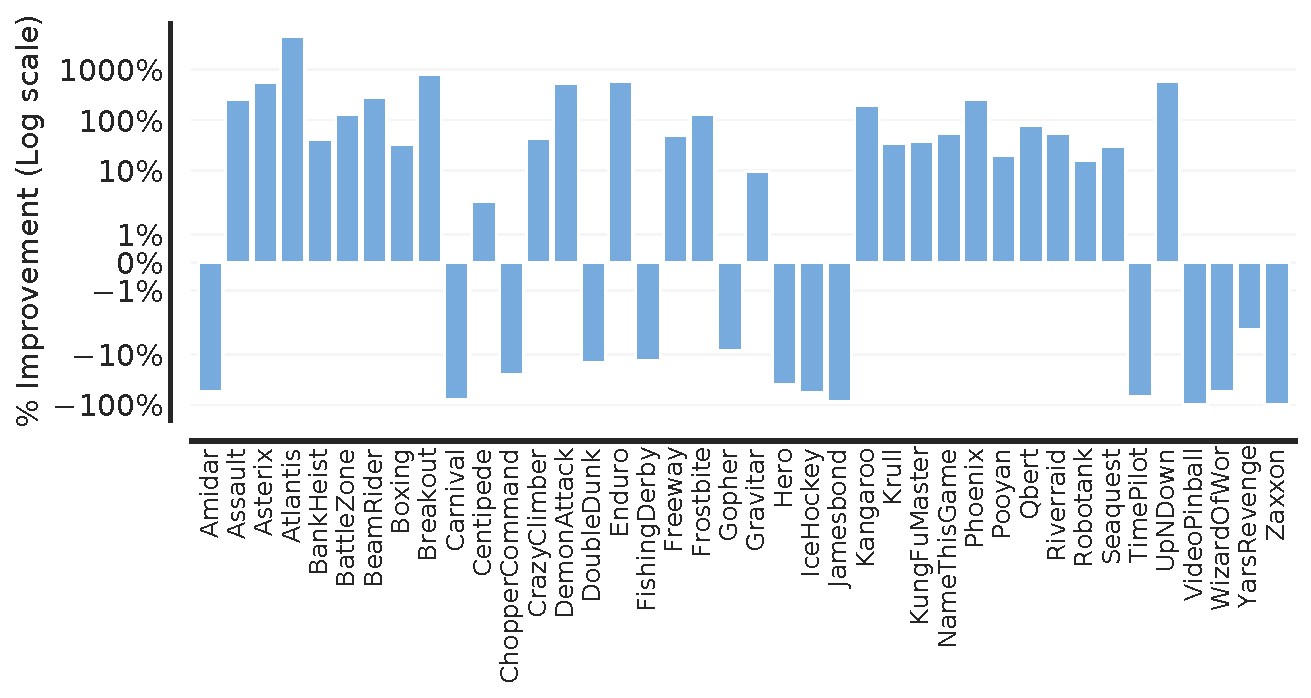
\includegraphics[width=\linewidth]{chapters/scaled_ql/figures/percent_improvement_over_DT.pdf}
    \end{minipage}
    \hfill
    \begin{minipage}{0.34\linewidth}
    \vspace{-0.2cm}
 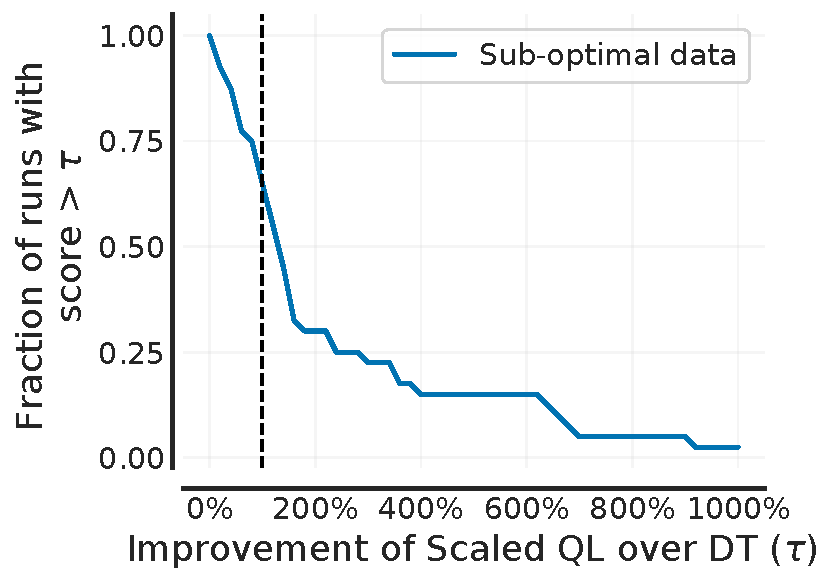
\includegraphics[width=\linewidth]{chapters/scaled_ql/figures/pp_profile_ql_dt.pdf}
    \end{minipage}
    \vspace{-0.4cm}
    \caption{\textbf{Comparing Scaled QL to DT} on all training games on the sub-optimal dataset.}
    \label{fig:percent_improvement}
    \vspace{-0.5cm}
\end{figure}

In our experiments, we study how our approach, scaled Q-learning, can simultaneously learn from sub-optimal and optimal data collected from 40 different Atari games. 
We compare the resulting multi-task policies to behavior cloning~(BC) with same architecture as scaled QL, and the prior state-of-the-art method based on decision transformers (DT)~\citep{chen2021decision}, which utilize return-conditioned supervised learning with large transformers~\citep{lee2022multi}, and have been previously proposed for addressing this task. 
We also study the efficacy of the multi-task initialization produced by scaled Q-learning in facilitating rapid transfer to new games via both offline and online fine-tuning, in comparison to state-of-the-art self-supervised representation learning methods and other prior approaches. Our goal is to answer the following questions: \textbf{(1)} How do our proposed design decisions impact performance scaling with high-capacity models?, \textbf{(2)} Can scaled QL more effectively leverage higher model capacity compared to na\"ive instantiations of Q-learning?, \textbf{(3)} Do the representations learned by scaled QL transfer to new games? We will answer these questions in detail through multiple experiments in the coming sections, but we will first summarize our main results below.


\textbf{Main empirical findings.} Our main results are summarized in Figures~\ref{fig:suboptimal_offline} and \ref{fig:main_results}. These figures show the performance of scaled QL, multi-game decision transformers~\citep{lee2022multi} (marked as ``DT''), a prior method based on supervised learning via return conditioning, and standard behavioral cloning baselines (marked as ``BC'') in the two settings discussed previously, where we must learn from: (i) near optimal data, and (ii) sub-optimal data obtained from the initial 20\% segment of the replay buffer (see our discussion about the problem setup). See Figure~\ref{fig:percent_improvement} for a direct comparison between DT and BC.


\begin{wrapfigure}{r}{0.5\linewidth}
    \vspace{-0.5cm}
    \centering
    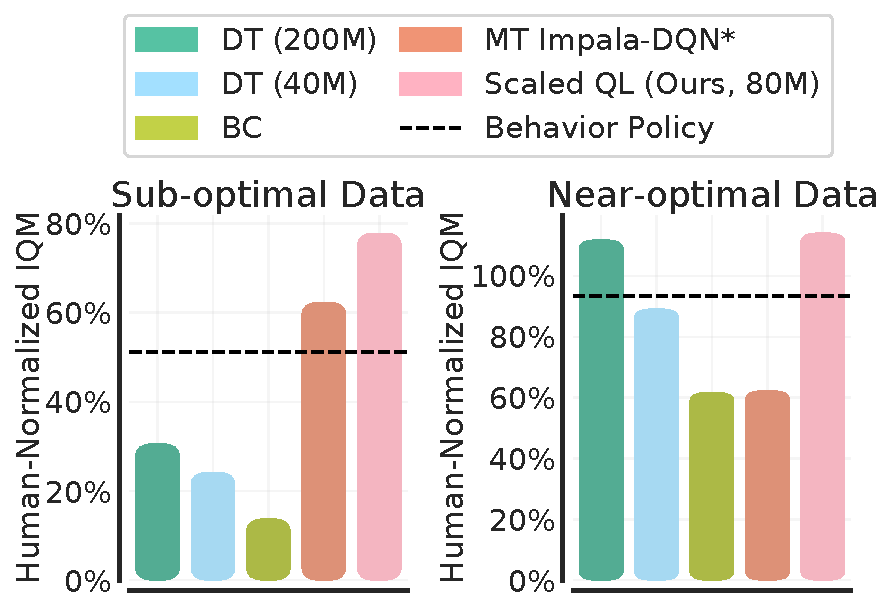
\includegraphics[width=0.95\linewidth]{chapters/scaled_ql/combnined_data_results_iqm.pdf}
    \vspace{-0.25cm}
    \caption{\footnotesize{\textbf{Offline scaled conservative Q-learning vs other prior methods} with near-optimal data and sub-optimal data. Scaled QL outperforms the best DT model, attaining an IQM human-normalized score of \textbf{114.1\%} on the near-optimal data and \textbf{77.8\%} on the sub-optimal data, compared to 111.8\% and 30.6\% for DT, respectively.}}
    \label{fig:main_results}
    \vspace{-0.5cm}
\end{wrapfigure}

In the more challenging sub-optimal data setting, scaled QL attains a performance of \textbf{77.8\%} IQM human-normalized score, although trajectories in the sub-optimal training dataset only attain 51\% IQM human-normalized score. Scaled QL also outperforms the prior DT approach by \textbf{2.5 times} on this dataset, even though the DT model has more than twice as many parameters and uses data augmentation, compared to scaled QL. 

In the $2^{nd}$ setting with near-optimal data, where the training dataset already contains expert trajectories, scaled QL with 80M parameters still outperforms the DT approach with 200M parameters, although the gap in performance is small (3\% in IQM performance, and 20\% on median performance). 
Overall, these results show that scaled QL is an effective approach for learning from large multi-task datasets, for a variety of data compositions including sub-optimal datasets, where we must stitch useful segments of suboptimal trajectories to perform well, and near-optimal datasets, where we should attempt to mimic the best behavior in the offline dataset. 

To the best of our knowledge, these results represent the largest performance improvement over the average performance in the offline dataset on such a challenging problem. We will now present experiments that show that offline Q-learning scales and generalizes.

\begin{figure}[h]
\centering
\vspace{-0.2cm}
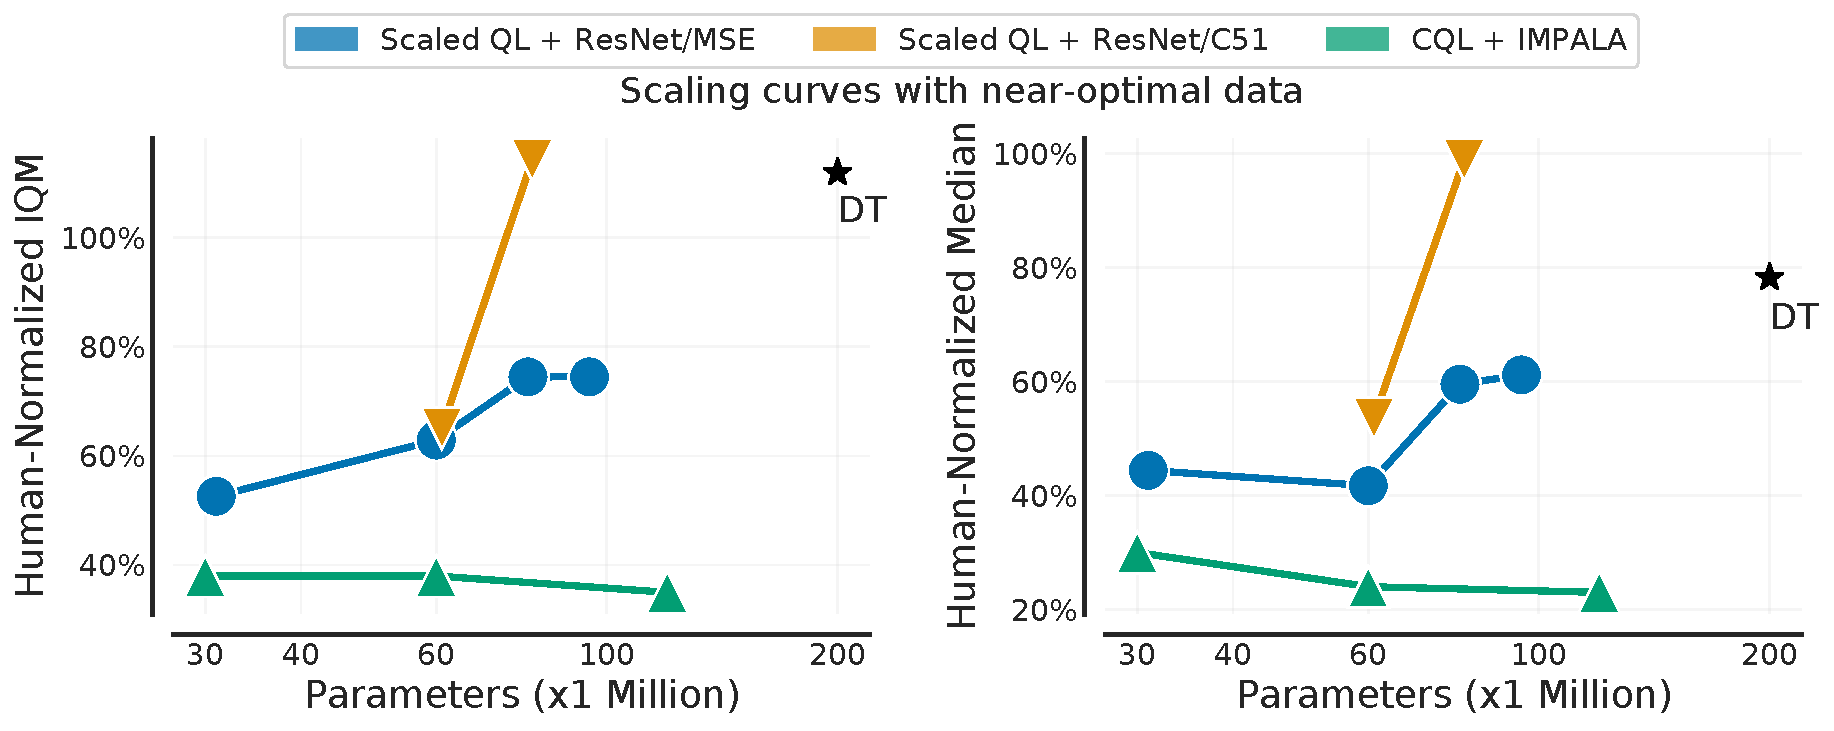
\includegraphics[width=0.75\linewidth]{chapters/scaled_ql/figures/scaling_plot_params_with_dt.pdf}
\vspace{-0.2cm}
\caption{\footnotesize{\textbf{Scaling trends for offline Q-learning.} Observe that while the performance of scaled QL instantiated with IMPALA architectures~\citep{espeholt2018impala} degrades as we increase model size, the performance of scaled QL utilizing the ResNets described in Section~\ref{sec:scaledql_method} continues to increase as model capacity increases. This is true for both an MSE-style TD error as well as for the categorical TD error used by C51 (which performs better on an absolute scale). The CQL + IMPALA performance numbers are from~\citep{lee2022multi}.}
}
\label{fig:scaling}
\vspace{-0.2cm}
\end{figure}

\vspace{-0.2cm}
\subsubsection{Does Offline Conservative Q-Learning Scale Favorably?}
\vspace{-0.2cm}
One of the primary goals of this chapter was to understand if scaled Q-learning is able to leverage the benefit of higher capacity architectures. Recently, \citet{lee2022multi} found that the performance of CQL with the IMPALA architecture does not improve with larger model sizes and may even degrade with larger model sizes. To verify if scaled Q-learning can address this limitation, we compare our value-based offline RL approach with a variety of model families: \textbf{(a)} IMPALA family~\citep{espeholt2018impala}: three IMPALA models with varying widths ($4, 8, 16$) whose performance numbers are taken directly from \citet{lee2022multi} (and was consistent with our preliminary experiments), 
%%AK: check if this is the standard naming or not?
\textbf{(b)} ResNet 34, 50, 101 and 152 from the ResNet family, modified to include group normalization and learned spatial embeddings.%, and \textbf{(c)} ViT-Base and ViT-Large from the vision transformer family, similar to decision transformers. 
These architectures include both small and large networks, spanning a wide range from 1M to 100M parameters. As a point of reference, we use the scaling trends of the multi-game decision transformer and BC approaches from \citet{lee2022multi}.
%%SL.9.27: if we don't end up including vit, make sure to revise the above discussion

Observe in Figure~\ref{fig:scaling} that the performance of scaled Q-learning improves as the underlying Q-function model size grows. Even though the standard mean-squared error formulation of TD error results in worse absolute performance than C51 (blue vs orange), for both of these versions, the performance of scaled Q-learning increases as the models become larger. This result indicates that value-based offline RL methods can scale favorably, and give rise to better results, but this requires carefully picking a model family. This also explains the findings from \citet{lee2022multi}: while this prior work observed that CQL with IMPALA scaled poorly as model size increases, they also observed that the performance of return-conditioned RL instantiated with IMPALA architectures also degraded with higher model sizes. Combined with the results in Figure~\ref{fig:scaling} above, this suggests that poor scaling properties of offline RL can largely be attributed to the choice of IMPALA architectures, which may not work well in general even for supervised learning methods (like return-conditioned BC).


\vspace{-0.2cm}
\subsubsection{Can Offline RL Learn Useful Initializations that Enable Fine-Tuning?}
\label{sec:ft_off_on}
\vspace{-0.2cm}

Next, we study how multi-task training on multiple games via scaled QL can learn general-purpose representations that can enable \emph{rapid} fine-tuning to new games. We study this question in two scenarios: fine-tuning to a new game via offline RL with a small amount of held-out data (1\% uniformly subsampled datasets from DQN-Replay~\citep{agarwal2019optimistic}), and finetuning to a new game mode via sample-efficient online RL initialized from our multi-game offline Q-function. For finetuning, we transfer the weights from the visual encoder and reinitialize the downstream feed-forward component (Figure~\ref{fig:overview}). For both of these scenarios, we utilize a ResNet101 Q-function trained via the methodology in Section~\ref{sec:scaledql_method}, using C51 and feature normalization.

\begin{figure}[t]
    \centering
    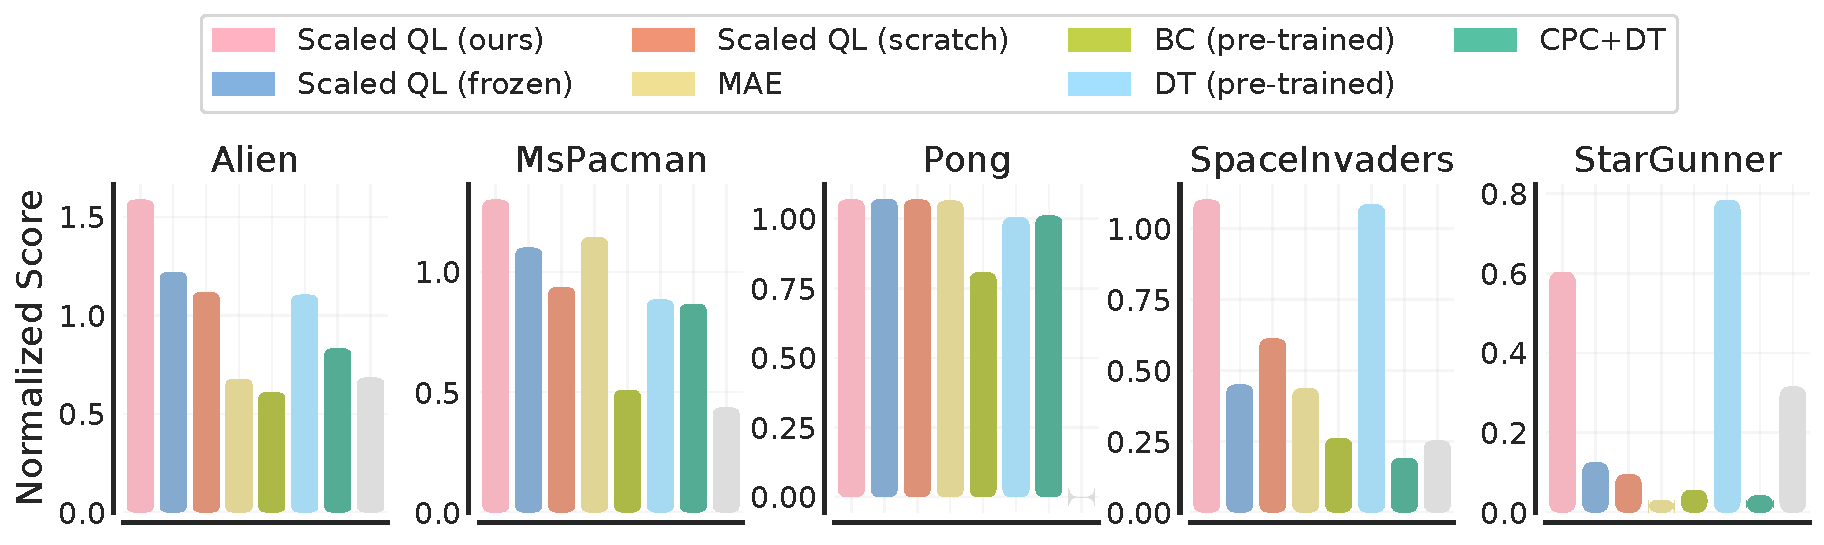
\includegraphics[width=0.99\linewidth]{chapters/scaled_ql/figures/offline_ft.pdf}
    \vspace{-0.25cm}
    \caption{\footnotesize{\textbf{Offline fine-tuning} performance on unseen games trained with 1\% of held-out game's data, measured in terms of DQN-normalized score, following \citep{lee2022multi}. On average, pre-training with scaled QL outperforms other methods by \textbf{82\%}. Furthermore, scaled QL improves over scaled QL (scratch) by 45\%, indicating that the representations learned by scaled QL during multi-game pre-training are useful for transfer. Self-supervised representation learning (CPC, MAE) alone does not attain good fine-tuning performance.}}
    \label{fig:offline_ft}
    \vspace{-0.3cm}
\end{figure}
%%AK: not having baselines para here, since the comparisons are different

\textbf{Scenario 1 (Offline fine-tuning)}: First, we present the results for fine-tuning in an offline setting: following the protocol from \citet{lee2022multi}, we use the pre-trained representations to rapidly learn a policy for a novel game using limited offline data (1\% of the experience of an online DQN run). In Figure~\ref{fig:offline_ft}, we present our results for offline fine-tuning on 5 games from \citet{lee2022multi}, \textsc{Alien, MsPacman, Space Invaders, StarGunner} and \textsc{Pong}, alongside the prior approach based on decision transformers (``DT (pre-trained)''), and fine-tuning using pre-trained representations learned from state-of-the-art self-supervised representation learning methods such as contrastive predictive coding (CPC)~\citep{oord2018representation} and masked autoencoders (MAE)~\citep{he2111masked}. For CPC performance, we use the baseline reported in \citet{lee2022multi}. MAE is a more recent self-supervised approach that we find generally outperformed CPC in this comparison. For MAE, we first pretrained a vision transformer~(ViT-Base)~\citep{dosovitskiy2020image} encoder with 80M parameters trained via a reconstruction loss on observations from multi-game Atari dataset and freeze the encoder weights as done in prior work~\citep{xiao2022masked}. 
Then, with this frozen visual encoder, we used the same feed forward architecture, Q-function parameterization, and training objective (CQL with C51) as scaled QL to finetune the MAE network. We also compare to baseline methods that do not utilize any multi-game pre-training (DT (scratch) and Scaled QL (scratch)). 

\textbf{Results.} Observe in Figure~\ref{fig:offline_ft} that multi-game pre-training via scaled QL leads to the best fine-tuning performance and improves over prior methods, including decision transformers trained from scratch. %, by XX\% in aggregate. 
Importantly, we observe \emph{positive transfer} to new games via scaled QL. Prior works~\citep{badia2020agent57}
running multi-game Atari (primarily in the online setting) have generally observed negative transfer across Atari games. We show for the first time that pre-trained representations from Q-learning enable positive transfer to novel games that significantly outperforms return-conditioned supervised learning methods and dedicated representation learning approaches.

\textbf{Scenario 2 (Online fine-tuning)}: Next, we study the efficacy of the learned representations in enabling online fine-tuning. While deep RL agents on ALE are typically trained on default game modes~(referred to as $m0d0$), we utilize new \emph{variants} of the ALE games designed to be challenging for humans~\citep{machado18sticky} for online-finetuning. We investigate whether multi-task training on the 40 default game variants can enable fast online adaptation to these never-before-seen variants. In contrast to offline fine-tuning (Scenario 1), this setting tests whether scaled QL can also provide a good initialization for online data collection and learning, for closely related but different tasks. Following \citet{farebrother2018generalization}, we use the same \emph{variants} investigated in this prior work: $\textsc{Breakout}$, $\textsc{Hero}$, and $\textsc{Freeway}$, which we visualize in Figure~\ref{fig:online_ft}~(left).
To disentangle the performance gains from multi-game pre-training and the choice of Q-function architecture, we compare to a baseline approach (``scaled QL (scratch)'') that utilizes an identical Q-function architecture as pre-trained scaled QL, but starts from a random initialization. As before, we also evaluate fine-tuning performance using the representations obtained via masked auto-encoder pre-training~\citep{he2111masked,xiao2022masked}. We also compare to a single-game DQN performance attained after training for 50M steps, $16\times$ more transitions than what is allowed for scaled QL, as reported by \citet{farebrother2018generalization}.

\textbf{Results}. Observe in Figure~\ref{fig:online_ft} that fine-tuning from the multi-task initialization learned by scaled QL significantly outperforms training from scratch as well as the single-game DQN run trained with \textbf{16x} more data. Fine-tuning with the frozen representations learned by MAE performs poorly, which we hypothesize is due to differences in game dynamics and subtle changes in observations, which must be accurately accounted for in order to learn optimal behavior~\citep{dean2022don}. Our results confirm that offline Q-learning can both effectively benefit from higher-capacity models and learn multi-task initializations that enable sample-efficient transfer to new games. 


\begin{figure}[t]
    \centering
        
\includegraphics[width=0.9\linewidth]{chapters/scaled_ql/figures/legend_online_ft.pdf}
        \vspace{-0.1cm}
        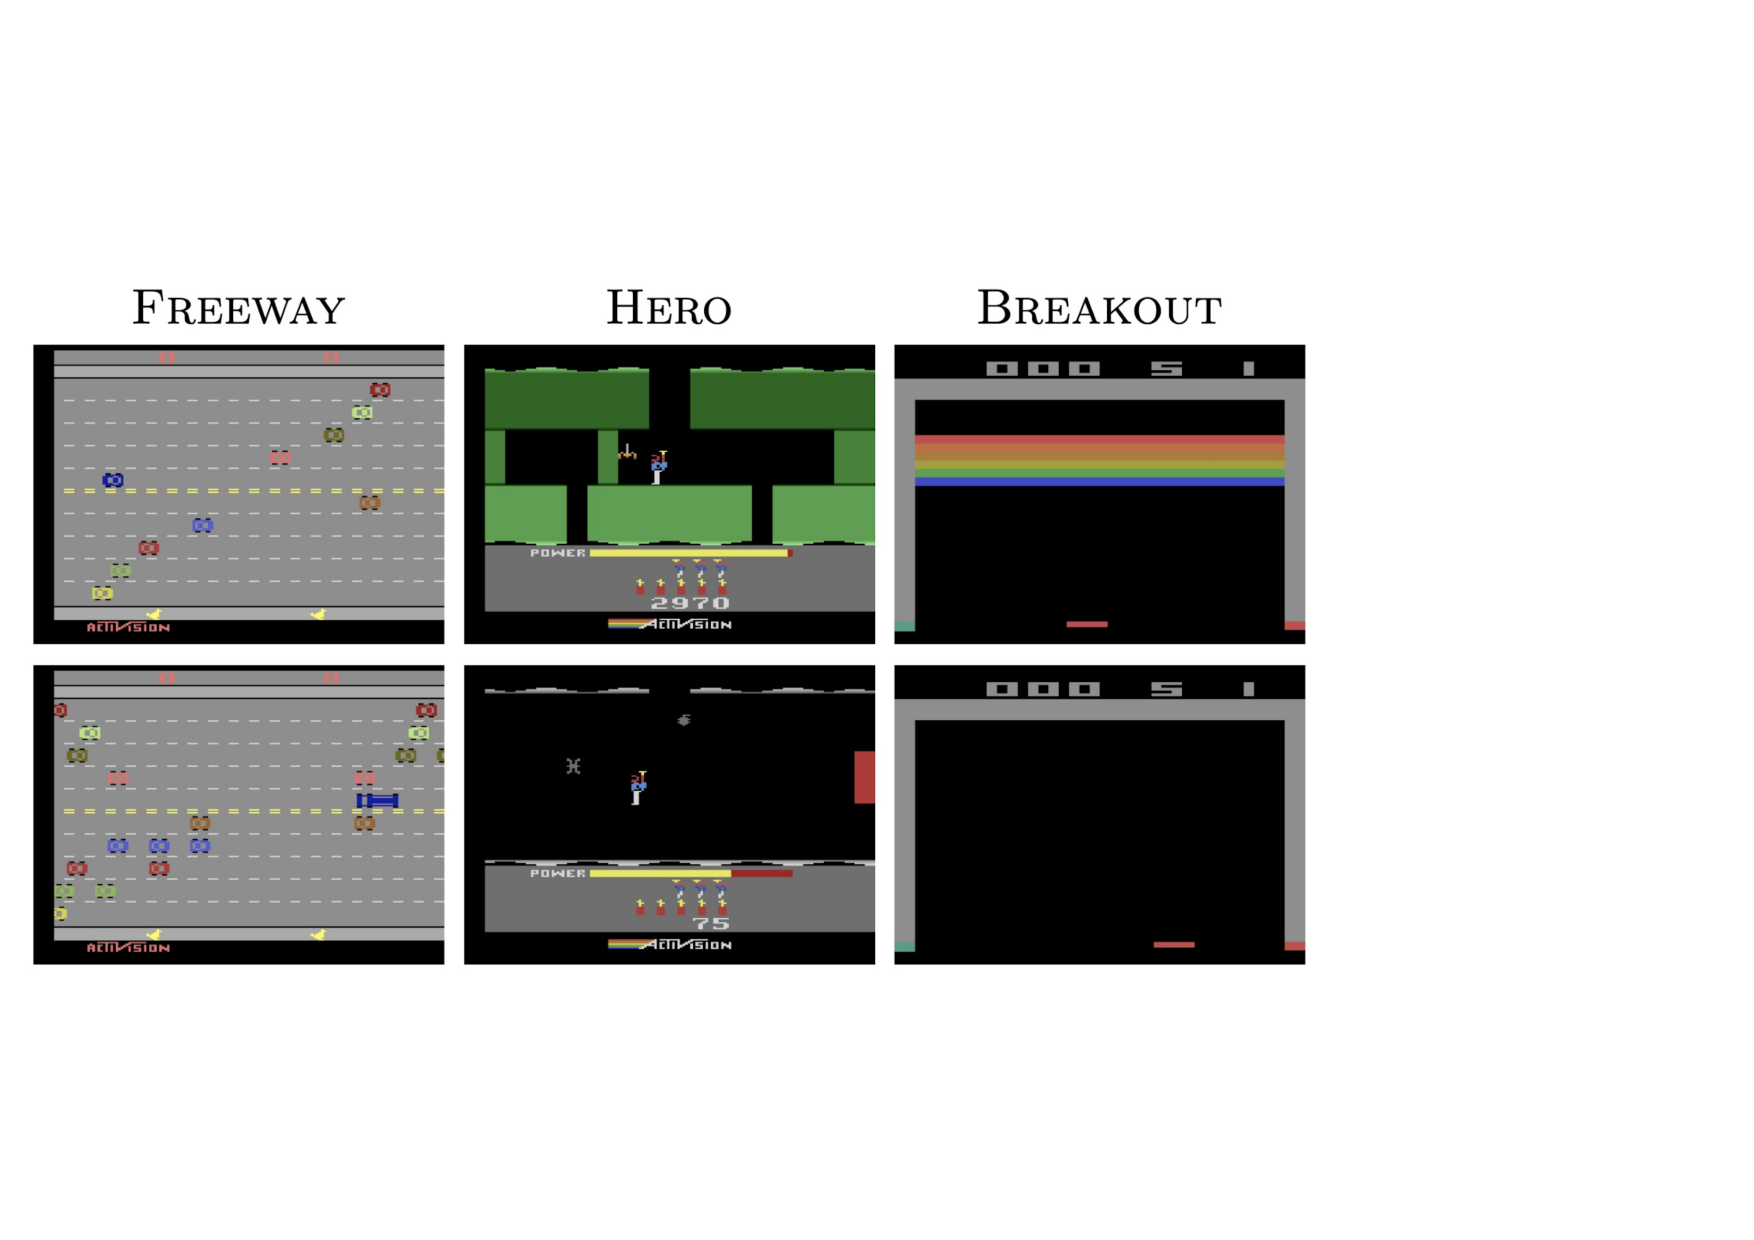
\includegraphics[width=0.35\linewidth]{chapters/scaled_ql/figures/atari_modes_3games.pdf}
        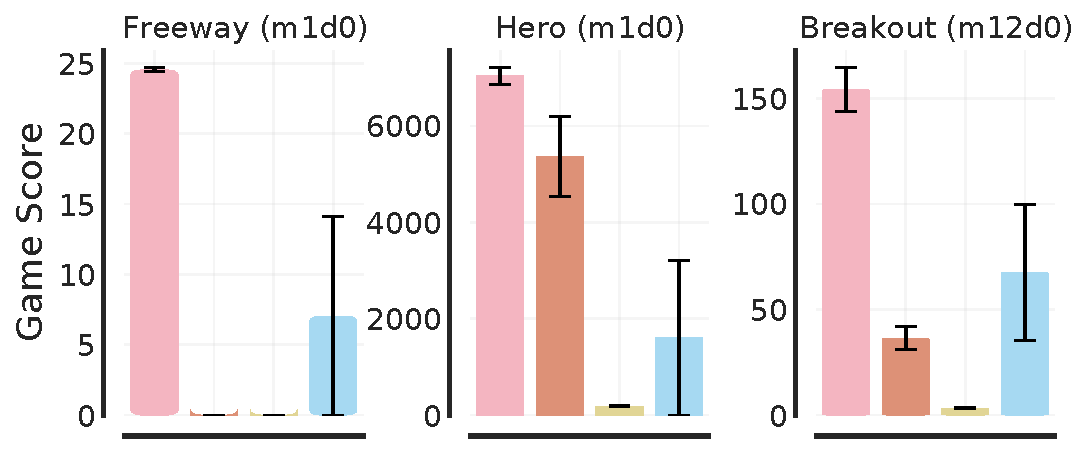
\includegraphics[width=0.5\linewidth]{chapters/scaled_ql/figures/online_ft_3_games.pdf}
    \vspace{-0.1cm}
    \caption{\footnotesize{\textbf{Online fine-tuning} results on unseen game \emph{variants}. \textbf{Left}. The top row shows default variants and the bottom row shows unseen variants evaluated for transfer: Freeway’s mode 1 adds buses, more vehicles, and increases velocity; Hero’s mode 1 starts the agent at level 5; Breakout’s mode 12 hides all bricks unless the ball has recently collided with a brick. \textbf{Right}. We fine-tune all methods except single-game DQN for 3M online frames (as we wish to test fast online adaptation). Error bars show minimum and maximum scores across 2 runs while the bar shows their average. Observe that scaled QL significantly outperforms learning from scratch and single-game DQN with 50M online frames. Furthermore, scaled QL also outperforms RL fine-tuning on representations learned using masked auto-encoders. See Figure~\ref{fig:lr_curves_online_ft} for learning curves.}}
    \label{fig:online_ft}
    \vspace{-0.5cm}
\end{figure}


\vspace{-0.25cm}
\subsubsection{Ablation Studies}
\label{sec:ablation}
\vspace{-0.25cm}

Finally, in this section we perform controlled ablation studies to understand how crucial the design decisions introduced in Section~\ref{sec:scaledql_method} are for the success of scaled Q-learning. In particular, we will attempt to understand the benefits of using C51 and feature normalization.

\textbf{MSE vs C51:} We ran scaled Q-learning with identical network architectures (ResNet 50 and ResNet 101), with both the conventional squared error formulation of TD error, and compare it to C51, which our main results utilize. Observe in Table~\ref{tab:ablation_mse} that C51 leads to much better performance for both ResNet 50 and ResNet 101 models. The boost in performance is the largest for ResNet 101, where C51 improves by over \textbf{39\%} as measured by median human-normalized score. This observation is surprising since prior work~\citep{agarwal2021deep} has shown that C51 performs on par with standard DQN with an Adam optimizer, which all of our results use. One hypothesis is that this could be the case as TD gradients would depend on the scale of the reward function, and hence some games would likely exhibit a stronger contribution in the gradient. This is despite the fact that our implementation of MSE TD-error already attempts to correct for this issue by applying the unitary scaling technique from \citep{kurin2022defense} to standardize reward scales across games. That said, we still observe that C51 performs significantly better.

\begin{table}[t]
    \centering
% \fontsize{8}{8}\selectfont
    \centering
    \vspace{-0.3cm}
    \caption{\footnotesize{\textbf{Performance of Scaled QL with the standard mean-squared TD-error and C51} in the offline 40-game setting aggregated by the median human-normalized score. Observe that for both ResNet 50 and ResNet 101, utilizing C51 leads to a drastic improvement in performance.}}% (as large as 39.4\% improvement on human-median normalized score with ResNet 101).}}
    \label{tab:ablation_mse}
    \vspace{0.1cm}
\resizebox{0.6\linewidth}{!}{\begin{tabular}{lcc}
\toprule
 & \textbf{Scaled QL (ResNet 50)} & \textbf{Scaled QL (ResNet 101)} \\
\midrule
\textbf{with MSE}  &  41.1\% & 59.5\%  \\
\midrule
\textbf{with C51}  & 53.5\% (+12.4\%) & 98.9\% (+39.4\%) \\
\bottomrule
\vspace{-0.25in}
\end{tabular}}
\end{table}


\textbf{Importance of feature normalization:} We ran small-scale experiments with and without feature normalization (Section~\ref{sec:scaledql_method}). In these experiments, we consider a multi-game setting with only 6 games: \textsc{Asterix}, \textsc{Breakout}, \textsc{Pong}, \textsc{SpaceInvaders}, \textsc{Seaquest}, and we train with the initial 20\% data for each game. We report aggregated median human-normalized score across the 6 games in Table~\ref{tab:ablation_dr3} for three different network architectures (ResNet 34, ResNet 50 and ResNet 101). Observe that the addition of feature normalization significantly improves performance for all the models. Motivated by this initial empirical finding, we used feature normalization in all of our main experiments. Overall, the above ablation studies validate the efficacy of the two key design decisions in this chapter. 
% However, there are several avenues for future investigation: 1) it is unclear if C51 works better because of the distributional formulation or the categorical representation and experiments with other distributional formulations could answer this question, 2) we did not extensively try alternate feature normalization schemes which may improve results. 

\begin{table}[ht]
    \centering
% \fontsize{8}{8}\selectfont
    \centering
    \vspace{-0.2cm}
    \caption{\footnotesize{\textbf{Performance of Scaled QL with and without feature normalization in the 6 game setting} reported in terms of the median human-normalized score. Observe that with models of all sizes, the addition of feature normalization improves performance.}}
    \label{tab:ablation_dr3}
    \vspace{0.1cm}
\resizebox{\linewidth}{!}{\begin{tabular}{lccc}
\toprule
 & \textbf{Scaled QL (ResNet 34)} & \textbf{Scaled QL (ResNet 50)} & \textbf{Scaled QL (ResNet 101)} \\
\midrule
\textbf{without feature normalization}  &  50.9\%  & 73.9\% & 80.4\%    \\
\midrule
\textbf{with feature normalization}  & 78.0\% (+28.9\%)  & 83.5\% (+9.6\%)  & 98.0\% (+17.6\%) \\
\bottomrule
\vspace{-0.2in}
\end{tabular}
}
\end{table}

\textbf{Additional ablations:} We also conducted ablation studies for the choice of the backbone architecture (spatial learned embeddings) in Appendix~\ref{app:backbone_ablation}, and observed that utilizing spatial embeddings is better. We also evaluated the performance of scaled QL without conservatism to test the importance of utilizing pessimism in our setting with diverse data in Appendix~\ref{app:no_pessimism}, and observe that pessimism is crucial for attaining good performance on an average. We also provide some scaling studies for another offline RL method (discrete BCQ) in Appendix~\ref{app:discrete_bcq}.
%\input{applications}
\documentclass[../thesis.tex]{subfiles}
\begin{document}
In this thesis, we have presented a number of advances towards learning based 3D object reconstruction. In Chapter \ref{chapter:CategoryShapes}, we presented an algorithm to learn category-specific deformable 3D models for diverse object categories and showed how to use them in conjunction with recognition systems to achieve fully automatic object localization and reconstruction from a single image. In Chapter \ref{chapter:Amodal}, we worked towards calibrating the size of the reconstructed objects by inferring their relative sizes and depths from a single image. We did this by leveraging amodal bounding boxes and reasoning about object co-occurences in image collections. We worked towards unifying single and multi-view reconstruction with a CNN in Chapter \ref{chapter:LSM} with Learnt Stereo Machines.

We have still just scratched the tip of the iceberg as alluded to in the limitations of current works in the chapters above. A number of challenges remain in tightly integrating semantic reasoning and 3D reconstruction (some of which we summarize below) and present for exciting directions for future work. 

\paragraph{Shape Representations:} In our works, we have explored using deformable meshes, voxel occupancy grids and depth maps as representations for shape. While each presents its own benefits, it is still unclear whether one has all the desirable properties for shape representations. For example, part compositionality plays a crucial role in the human visual system which none of the above representations exhibit. There have been promising works towards modelling shapes with primitives such as planes and simple shapes~\cite{abstractionTulsiani17} (cubes, cylinders \etc). Automatic discovery of such primitives which can be shared across object categories would allow for greater interpretability in reconstructions.

\paragraph{Learning without explicit supervision:} We, as humans, almost never have ``ground truth'' data to learn from - especially for 3D shapes. Our mental models are built from observing objects from different viewpoints, in various lighting conditions, by interacting with them \etc This remains a critical problem to solve for current learning systems to scale beyond available 3D datasets. Some recent works~\cite{tulsiani2017multi,zhou2017unsupervised} have investigated using motion and projection into novel views as a proxy for learning shapes. An exciting direction to investigate would be coupling active exploration with 3D shape inference. For example, a robot could derive shape cues for an object by trying to grasp/poke/manipulate it in certain ways.

\paragraph{Quality of reconstructions:} A common issue with current methods for learning-based shape inference methods is that they dont produce high quality outputs (in terms of accuracy, fidelity and resolution). This is in contrast with classical systems which produce extremely detailed models, albeit from far more images. Recent attempts at modelling high resolution grids with CNNs~\cite{hane2017hierarchical} present a promising direction towards detailed reconstructions with learning-based cues. A related task is modelling large spaces with such systems which couples with the question of what shape representations are amenable to such problems.

\paragraph{Related tasks:} While inferring 3D shape from 2D views is an end in itself, it can be especially useful for a number of complementary and upstream tasks. For example, estimating lighting and reflectance in scenes could benefit from learning-based 3D inference systems, particularly when learnt jointly~\cite{barronPAMI13}. More examples of properties for which are difficult to \textit{ground-truth} and tightly coupled with 3D reasoning are optical flow and scene flow. Learning systems could provide a very natural way of jointly modelling these variety of tasks with strong inter-dependencies. Implicit 3D reasoning could also play a critical role in end-to-end learning of policies in robotics~\cite{finn2016end}, \eg for navigating in 3D scenes or manipulating objects.

\end{document}
\section*{Acknowledgements}
This work was supported in part by NSF Award IIS-1212798 and ONR MURI-N00014-10-1-0933. Shubham Tulsiani was supported by the Berkeley fellowship and Jo\~{a}o Carreira was supported by the Portuguese Science Foundation, FCT, under grant SFRH/BPD/84194/2012. We gratefully acknowledge NVIDIA corporation for the donation of Tesla GPUs for this research.


{\small
\bibliographystyle{ieee}
\bibliography{referencesClean}
}

\end{document}
